\section{Design and Implementation}\label{sec:design}
In this chapter, I am going to describe the design and implementation steps realized for the demonstrator. Section \ref{subsec:exampleforimplementation} describes all the examples that I have conceptualized before choosing the final one for the implementation. This is then followed by the description of the steps taken for selecting the bx-tool in Section \ref{subsec:bxtoolselection}. Section \ref{subsec:architecturedesign} deals with the decisions taken for finalizing the application's architecture design. Section \ref{subsec:design_layers} describes the application's framework in detail along with its components. Finally, Section \ref{subsec:designchallenges} describes the challenges that I faced during the design and implementation of the entire framework. 

My demonstrator is called \textit{\ac{Demon-BX}}. Demon-BX is designed in such a way that the implementation is extensible for a family of (similar) examples, and for more than one bx tool. Due to time limitations and scope of this thesis, I chose one of each for the implementation process.

\subsection{Choosing an Example}\label{subsec:exampleforimplementation}
To solve the problems described in Section \ref{subsec:probstmt}, the main idea is to design and implement an interactive bx tool demonstrator based on an intuitive example.

\subsubsection{Construction}\label{subsubsec:exampleconstruction}
I have constructed a few examples as candidates for the implementation as follows:

\paragraph{Task Management} This idea is influenced from the project management tool such as \textit{Trello} (\url{https://trello.com/}), a web-based project management tool for organizing and managing project related work. This prototype can be used for allocating tasks in a team. It contains two views, a supervisor's view and an employee's view. A supervisor can allocate tasks to their subordinates. An employee can view only the tasks assigned to him. Then the task will go through a life cycle as the work progresses, i.e., Assigned, In Progress, Testing, Done. The supervisor's view shows aggregate information from multiple projects and multiple employees but does not contain detailed information, e.g., tasks have fewer states than for assigned employees. A bx controls how updates are handled and states are reflected in the different views of the project, e.g., the employee's view will be updated for each state change, whereas the supervisor's view is only updated when a task is completed and not for intermediate changes.

This example is well-known among the developer's community. But, the example contains a set of rules related to project management which is complex to operate on and user interaction does not come naturally with it. In this example, a user can relate to the bx concepts with both forward and backward synchronization, but it involves texts, tables etc. which is not intuitive for a user.

\paragraph{Quiz} This prototype can be used for an online quiz game. It contains two views, an administrator's view and a participant's view.
There will be a large set of questions related to different areas, e.g, history, geography, politics, sports, etc. The administrator can select the areas from which the questions will be shown to the participant and initiate the game. The participant can view the selection of the areas and start the quiz. Randomly questions will be shown to the participant from the selected areas with 4 options. The administrator's view contains less information than the participant's view, e.g., only the result of each question will be shown to the administrator, whereas participants can see questions along with its options. As soon as the participant chooses the answer to any question, a bx controls how updates are handled and states are reflected in the different views of the project.

Most of the students and computer game lovers are familiar with this example. But, the example contains a set of rules which a user first needs to understand before starting the game and user interaction does not come naturally with it. In this example, a user can relate to the bx concepts with both forward and backward synchronization, but it involves texts, menus, tables etc. which is not intuitive for a user.

\paragraph{Playing with Shapes} This prototype contains two views, a low-level view (depicts a \ac{UI} for a low-level language, i.e., a UI with less functionality) and a high-level view (depicts a UI for a high-level language, i.e., a UI with more functionality). The user will sketch a geometric shape, i.e., triangle/square/rectangle/circle using the low-level view. The high-level view tries to recognize the geometric shape and draws it precisely. A bx controls how updates are handled and states are reflected in the different views of the project. In the high-level view, more functionality will be available, e.g.,, moving one shape from one place to another, creating a clone of an existing shape, rotations, etc. which is not possible in low-level view.

This example is based on a new concept and hence contains rules which are completely new to the users. But user interaction is an integral part of this example. In this example, a user can relate to the bx concepts with both forward and backward synchronization and involves shapes, mouse movements etc. which are very interesting for a user.

\paragraph{Planning a Kitchen}
This prototype contains two views, layout view (depicts a grid structure containing blocks) and a symbolic view (empty space which depicts the UI for a kitchen). The symbolic view has more functionalities such as creating/deleting/moving a kitchen item, etc. out of which only a few will be available in the layout view. The user will create/delete/move a kitchen item, i.e., sink/table in the symbolic view and if changes are compatible with a bx then the items will be reflected in the layout view with colored blocks and vice-versa.

Any user can relate to this example very well as everybody is familiar with a kitchen and its environment. This example involves no technical details and simple rules as the environment is a part of day to day life and hence users will be able to relate to the learning concepts easily. As an integral part of this example, user interactivity involves shapes, colors, drag, and drop, etc. which creates interest for a user.

\paragraph{Families to Persons}
The concept of this example is taken from the example \emph{FamilyToPersons} located in the bx examples repository~\cite{bx-examples}. It contains two views, a Families view and a Persons view. The Families view contains many families and each family consist of members. The Persons view contains persons (corresponding to the members of each family). The addition of a new person to the Persons view will be reflected in the Families view and vice-versa. Surnames don't have to be unique. If a new person could be placed in multiple families the synchronizer can simply ask which one is to be chosen (user interaction).

The potential users are not familiar with this example. However, this example is very simple to understand as everybody is familiar with the concept of a family and hence users will be able to relate to the learning concepts easily. But user interactivity does not involve any colors, shapes, mouse movements, etc. to attract a user.

\subsubsection{Selection}\label{subsubsec:exampleselection}
Selecting an example for the demonstrator was not random, rather I have taken many factors into considerations before choosing the final one. It was a very important decision, as the selection of the example and its implementation will directly affect the research question \textit{RQ 4} specified in Section \ref{subsec:probstmt} and requirements \textit{NR2} (fun to play), \textit{NR3} (simple example) described in Section \ref{subsec:nonfunctionalreq}.

Hence by taking into account all these factors, I and my supervisor constructed a few evaluation criteria (referred to as \textbf{EC}), as due to time constraint, we could not ask potential users or conduct an experiment to find out what people will prefer. Then, we evaluated each example on the basis of the evaluation criteria for the selection of the most suitable example. The evaluation criteria that we have considered are listed below:
\begin{description}
	\item [EC 1:] User should be familiar with the example.
	\item [EC 2:] Example should be simple and intuitive with a minimum of technical details.
	\item [EC 3:] Interactivity should be a natural part of the example.
	\item [EC 4:] Both the forward and backward direction of consistency restoration should make sense for the example.
	\item [EC 5:] Example should be visual and involve shapes, colors and drag and drop (as opposed to text, menus, or tables).
\end{description}

Table~\ref{tab:comparison_examples} shows the comparison of the examples based on the evaluation criteria. "\checkmark" denotes the fulfillment of the evaluation criteria whereas, "\ding{55}" denotes the non-fulfillment of the evaluation criteria. This comparison table clearly shows that \textit{Planning a Kitchen} is the most suitable example as it fulfills all the evaluation criteria. So, I have finally chosen this example for the demonstrator and also as part of my research.

\begin{table}
	\centering
	\begin{tabular}{|lccccc|}
		\hline
		\textbf{} & \multicolumn{5}{c|}{\textbf{Evaluation Criteria}} \\
		\textbf{Examples} & \textbf{EC1} & \textbf{EC2} & \textbf{EC3} & \textbf{EC4} & \textbf{EC5} \\
		\hline
		\hline
		Task Management & \checkmark & \ding{55} & \ding{55} & \checkmark & \ding{55} \\ 
		\hline
		Quiz & \checkmark & \ding{55} & \ding{55} & \checkmark & \ding{55}\\
		\hline
		Playing with Shapes & \ding{55} & \ding{55} & \checkmark & \checkmark & \checkmark\\
		\hline
		Person and Family & \ding{55} & \checkmark & \checkmark & \checkmark & \ding{55}\\
		\hline
		Planning a Kitchen & \checkmark &  \checkmark & \checkmark & \checkmark & \checkmark \\
		\hline
	\end{tabular}
	\caption{Comparison of examples based on evaluation criteria}
	\label{tab:comparison_examples}
\end{table}

\subsection{BX Tool Selection}\label{subsec:bxtoolselection}
Next step in the design process was the selection of a bx tool which takes care of the bx part of the demonstrator and upon which the entire framework of the demonstrator will be constructed. Again, it was a very important decision, as the selection of the bx tool and the implementation on the top of it will directly affect the research questions \textit{RQ 1}, \textit{RQ 2}  specified in Section \ref{subsec:probstmt}.

My gathered information during the case study phase led the foundation for the selection process. I further investigated on the existing bx tools from the point of view of practical application and usage of these tools in terms of building software. Even after a significant amount of work has been done by developers community and bx community, the main problems were revolving around the conceptual, practical challenges associated with using bx, and tool/technology in building software systems and absence of benchmarks for comparison of complete bx solutions~\cite{bx-theoryandappl}.
To focus particularly on these issues, bx-community had conducted a series of technical workshops at relevant conferences and organized week-long intensive research seminars~\cite{bx-theoryandappl}. Some of the main outcomes of these seminars were (i) focus on the need of benchmarks and further categorizing them into functional and non-functional ones, (ii) software tool support for bx was shown in terms of demos which includes tool like eMoflon, Echo etc.

The outcome of the seminars led me to concentrate and analyze bx tools like eMoflon, Echo, BIGUL. Also, I came across the benchmark \cite{benchmarx} \cite{benchmarx-reload}, the first non-trivial benchmark where Anjorin et al. provide a practical framework to compare and evaluate three bx tools. After analyzing these tools, benchmarks and taking into consideration the research questions and requirements, I have finally chosen \textit{eMoflon} as the bx tool to handle the bx part of the demonstrator. Following were the driving factors for the selection of the bx tool:
\begin{itemize}
	\item {Anjorin et al. \cite{benchmarx-reload} tried to solve the main problem with benchmarking bx tools by creating a common design space, in which different bx tools architecture can be accommodated irrespective of the fact that they can have different input data. Hence, sample implementation with a fairly generic framework to implement the eMoflon tool was already available.}
	\item {my supervisor/prof. is a core member of the eMoflon developer team which gave me the added advantage of having good support. This extra knowledge actually helped me in solving the implementation issues/challenges related to the tool.}
	\item {eMoflon is Java based and was thus easier for me to integrate and work with, compared to e.g., BiGUL (Haskell-based), or NMF synchronization (C\# based).}
	\item {the technologies that I planned to use (JavaScript, Tomcat, servlets) during my implementation is also rather Java based.}
\end{itemize}

\subsection{Architecture Design}\label{subsec:architecturedesign}
The last step in the design process was application architecture design which is the most important part of my thesis and also the starting phase of the implementation of the prototype.

I decided to build a web application to address the requirements \textit{NR1} (minimal installation effort), \textit{NR6} (public access), \textit{NR7} (extendable), and \textit{NR8} (minimal requirements on user's environment) described in Section \ref{subsec:nonfunctionalreq}.

Web application development has evolved from single page design to very complex layering structures since the beginning of World Wide Web. Many design patterns \cite{designpattern} \cite{designpattern-notes} consisting of different technologies and programming languages were proposed, adopted and implemented to address the demands of customers and users on the web. With the rapid changes occurring on World Wide Web, some technologies are becoming obsolete and losing demand. Nowadays, the main trend appears to be improving user interaction and allowing developers to build powerful web applications rapidly.

I analyzed some design patterns and commonly used architecture designs by working on a few Proof of Concepts (PoC). The main goal of my thesis is to design and implement a demonstrator based on a bx-tool as described in Section \ref{subsec:contribution} and prior to this stage, I have already selected \textit{eMoflon} as my bx-tool in Section \ref{subsec:bxtoolselection}. The main idea was thus to check the feasibility of the architecture and the data flow within its components on top of the interface provided by the \textit{Benchmarx} framework (proposed by Anjorin et al. \cite{benchmarx-reload}) to access the bx-tool. While working on the PoCs, I encountered a few problems such as maintainability and reusability of code, dependencies of components etc. To avoid these problems and to address the requirement \textit{NREQ3} described in Section \ref{subsec:functionalreq}, I finally chose the Model-View-Controller (referred as \textbf{MVC} from now on) architecture for my application framework. Following were the driving factors for the selection of the MVC architecture \cite{designpattern-notes} \cite{designpattern-headfirst}:
\begin{itemize}
	\item {it differentiates the layers of a model, view, and controller for the re-usability and easy maintenance of code.}
	\item {it splits responsibilities into three main roles which allow developers to work independently without interfering in each other's work and for more efficient collaboration.}
	\item {due to the separation of concern, the same model can have any number of views. Enhancements in views and support of new technologies for building the view can be implemented easily.}
	\item {a person working on the view does not need to know about the underlying model code base and its architecture.}
\end{itemize}

\subsection{Architecture Layers}\label{subsec:design_layers}
This section provides an overview of the entire architecture followed by the description of each component e.g., Model, View, and Controller in detail.

\subsubsection{Overview}\label{subsubsec:design_overview}
The architecture has three components, Model, View and Controller to signify the MVC pattern. Figure~\ref{fig:Component_Diagram} describes the high-level architecture of the Demon-BX tool in the form of a component diagram.

\begin{figure}[h]
	\centering
	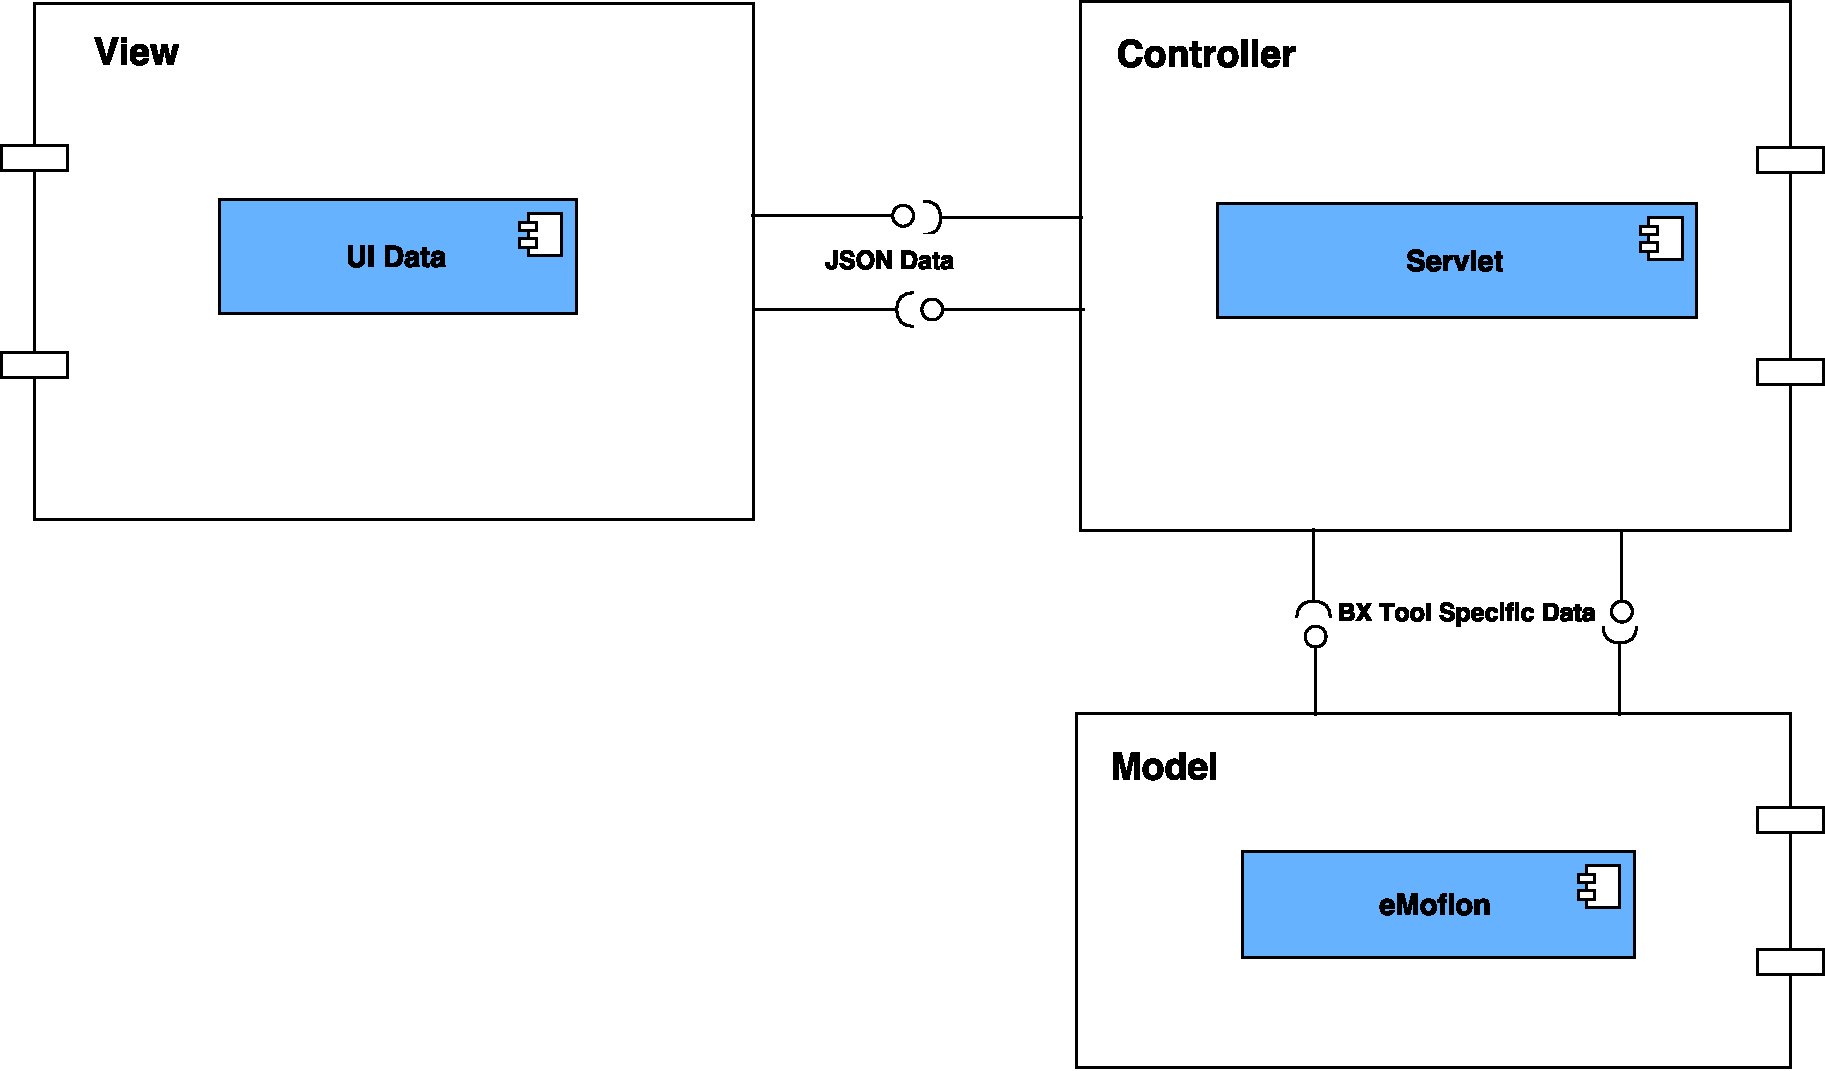
\includegraphics[width=1\textwidth]{figures/Component_Diagram-HighLevel}
	\caption{Component Diagram of Demon-BX Tool}
	\label{fig:Component_Diagram}
\end{figure}

The \texttt{model} component consists of a bx tool i.e., \texttt{eMoflon}, and a few Java classes encapsulating the implementation of the bx tool and transformation logic. It keeps all models and transformation rules, processes the data sent by the controller, and manages all tasks related to business logic, business rules, data, meta-models, state of meta-models, etc.

The \texttt{view} component contains a graphical user interface along with web technologies inside a web browser and a few Java classes. As a component, it is shown on a web browser as a part of a web application, provides an interface for a user to interact, and is responsible for capturing all user-related actions.

The \texttt{controller} component acts as a bridge between view and model and handles all user requests. It consists of a few Java classes. The controller receives all the user requests sent from the web browser and calls the appropriate methods where the actual data conversion happens, i.e., conversion of user data to example specific data before sending them to the bx tool for further processing, and conversion of example specific data to user data after receiving the processed data from the bx tool.

\begin{figure}
	\centering
	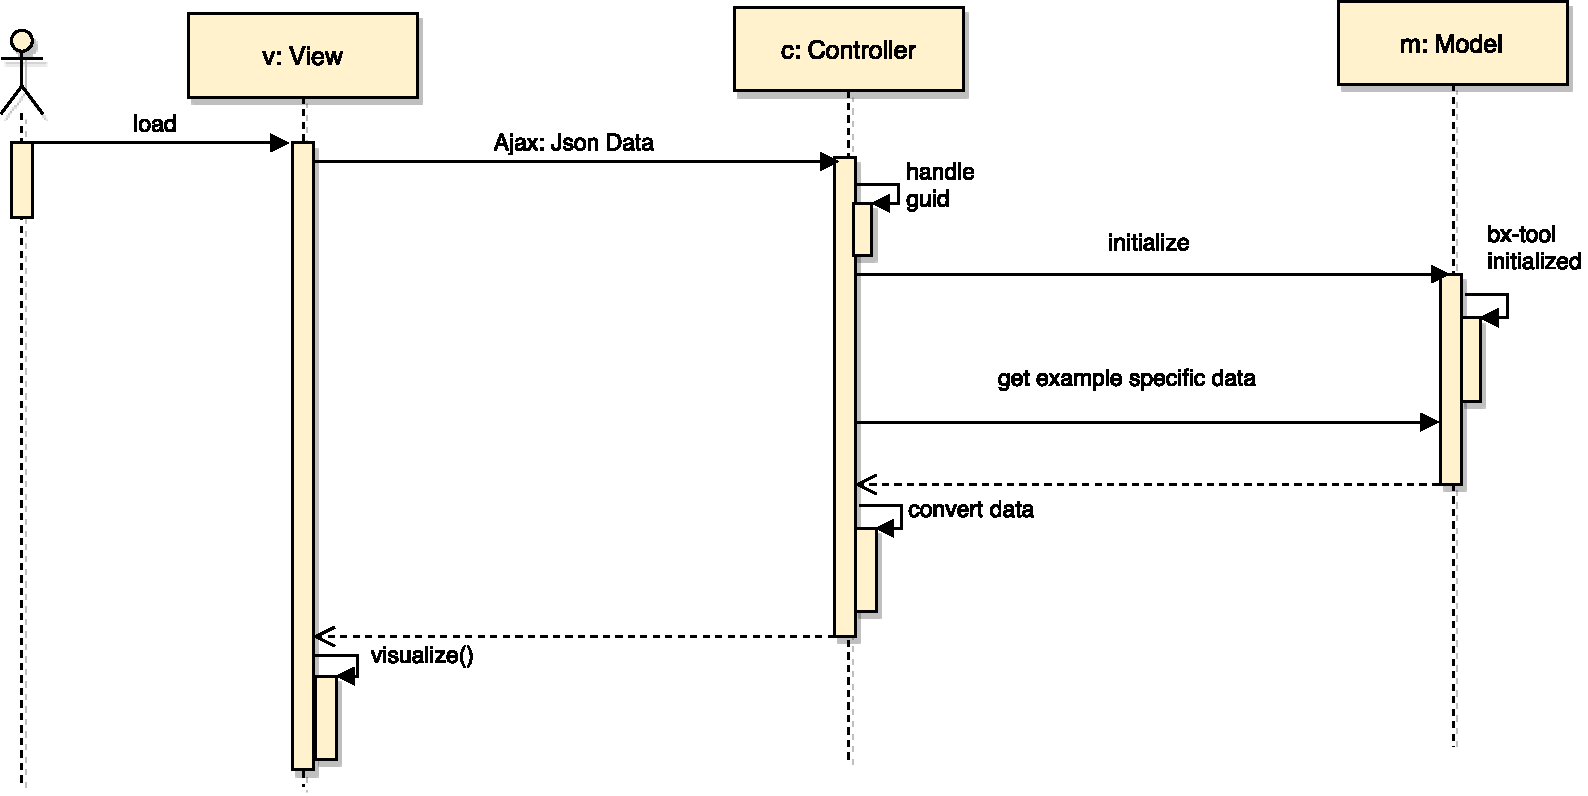
\includegraphics[width=1\textwidth]{figures/Sequence_Diagram-HighLevel(init)}
	\caption{Sequence Diagram of Demon-BX Tool: initialization}
	\label{fig:Sequence_Diagram-HighLevel(init)}
\end{figure}

\begin{figure}
	\centering
	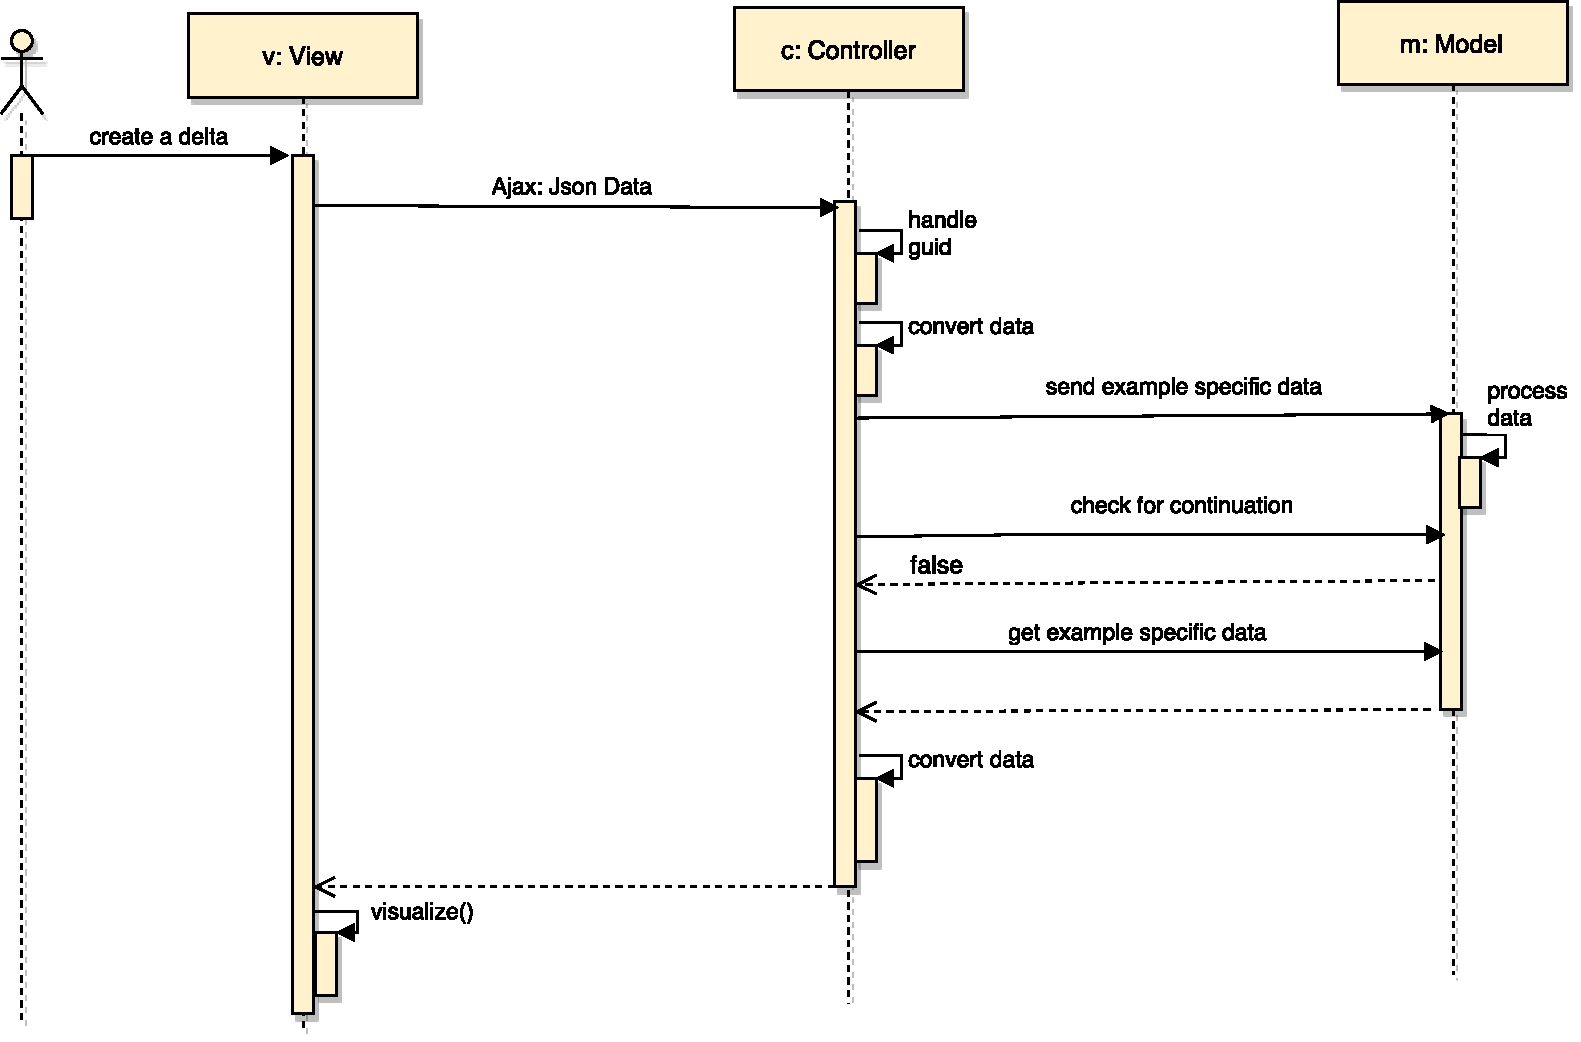
\includegraphics[width=1\textwidth]{figures/Sequence_Diagram-HighLevel(cont-false)}
	\caption{Sequence Diagram of Demon-BX Tool: delta propagation without continuation}
	\label{fig:Sequence_Diagram-HighLevel(cont-false)}
\end{figure}

\begin{figure}
	\centering
	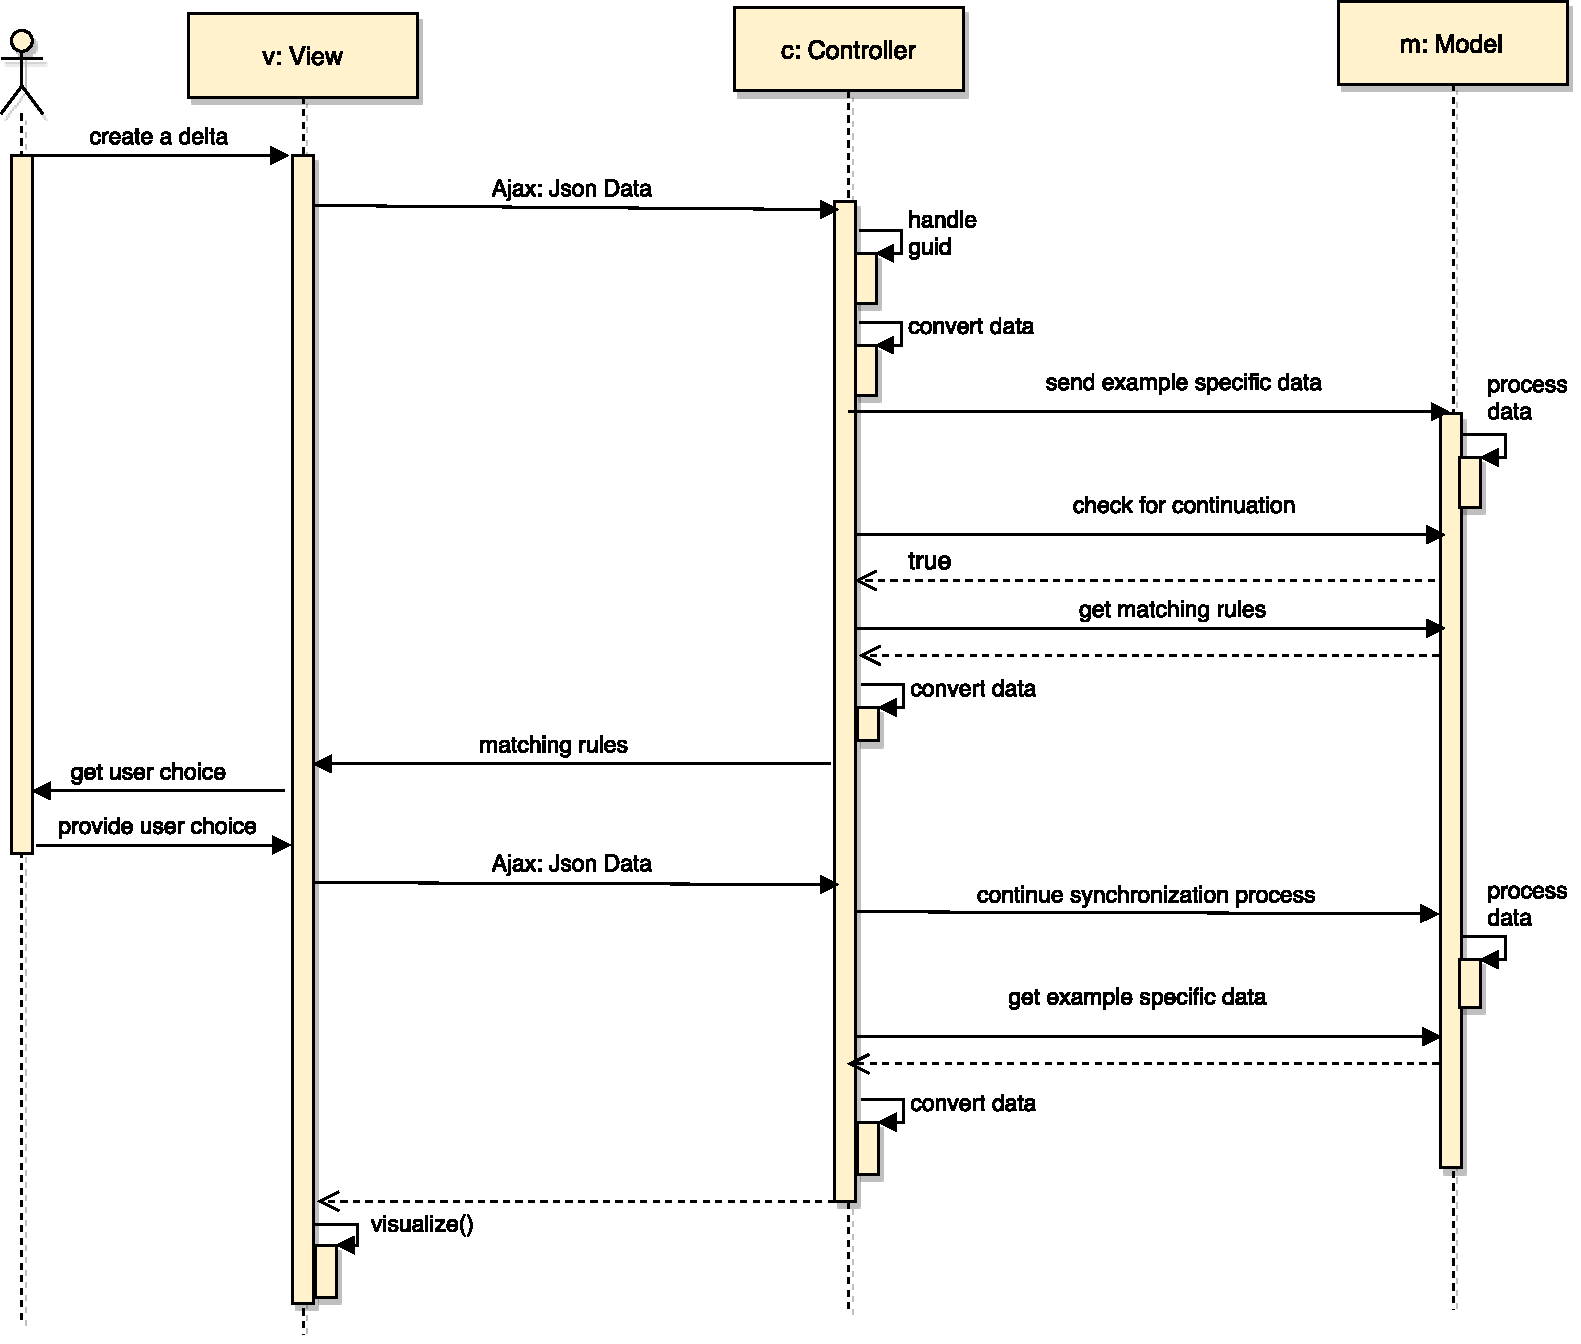
\includegraphics[width=1\textwidth]{figures/Sequence_Diagram-HighLevel(cont-true)}
	\caption{Sequence Diagram of Demon-BX Tool: delta propagation with continuation}
	\label{fig:Sequence_Diagram-HighLevel(cont-true)}
\end{figure}

\paragraph{Request-Response Cycle} 
The sequence diagrams shown in Figure~\ref{fig:Sequence_Diagram-HighLevel(init)}, Figure~\ref{fig:Sequence_Diagram-HighLevel(cont-false)}, Figure~\ref{fig:Sequence_Diagram-HighLevel(cont-true)} illustrate a high-level overview of the communication process between all three components in different stages.
\begin{enumerate}
	\item {\textbf{Load}: The user loads the application on a browser. The view generates a unique user id (GUID) and sends it to the controller as a request in the form of JSON data. After accepting the request, the controller stores the GUID and sends the initialize signal to the model for initializing the bx-tool. After tool gets initialized, the controller requests for the newly generated example specific models, converts it to the user data, and sends the response back to the view in the form of JSON data. The view processes the data and the final response is loaded into the browser. This entire process is shown in Figure~\ref{fig:Sequence_Diagram-HighLevel(init)}.}
	
	\item {\textbf{Delta Propagation (without continuation)}: After the application is loaded on the browser, the user creates a delta in one of the views and sends it to the controller along with the GUID generated earlier for the user as a request in the form of JSON data. After accepting the request, controller checks the existence of the GUID, converts the user data to the example specific data and sends it to the model for processing. During processing, the controller checks if satisfiability of more than one transformation rule exists for the processed data i.e., continuation. If continuation does not exist, the controller requests for the updated example specific models, converts it to the user data, and sends the response back to the view in the form of JSON data. The view processes the data and the final response is loaded into the browser. This entire process is shown in Figure~\ref{fig:Sequence_Diagram-HighLevel(cont-false)}.}
	
    \item {\textbf{Delta Propagation (with continuation)}: While the bx tool processes the delta, the controller checks if satisfiability of more than one transformation rule exists for the processed data i.e., continuation. If continuation exists, the controller gets the matching rules from the model, converts it to the user data, and sends it back to the view. The view asks the user for a choice. After the input is given by the user, the view sends it to the controller in the form of \texttt{JSON} data. The controller forwards the user's choice to the model and bx tool resumes processing of the data after getting it. After data is processed, 
    the controller requests for the updated example specific models, converts it to the user data, and sends the response back to the view in the form of JSON data. The view processes the data and the final response is loaded into the browser. This entire process is shown in Figure~\ref{fig:Sequence_Diagram-HighLevel(cont-true)}.}
\end{enumerate}

For better understanding and to avoid complexity, here I have described the delta propagation process for only a single delta. However, the user can generate multiple deltas as well. In that case, view collects all the deltas and sends them to the controller. After receiving the deltas, the controller handles them atomically (one by one).

\subsubsection{Model}\label{subsubsec:design_model}
The model is mainly responsible for encapsulating the access of data and handling the business logic of the application \cite{designpattern-headfirst} \cite{mvc-arch}. It ensures the data abstraction and provides methods to access it, due to which the complexity of writing the code on developers' part is highly reduced \cite{mdd-webwithmvc}.

\begin{figure}
	\centering
	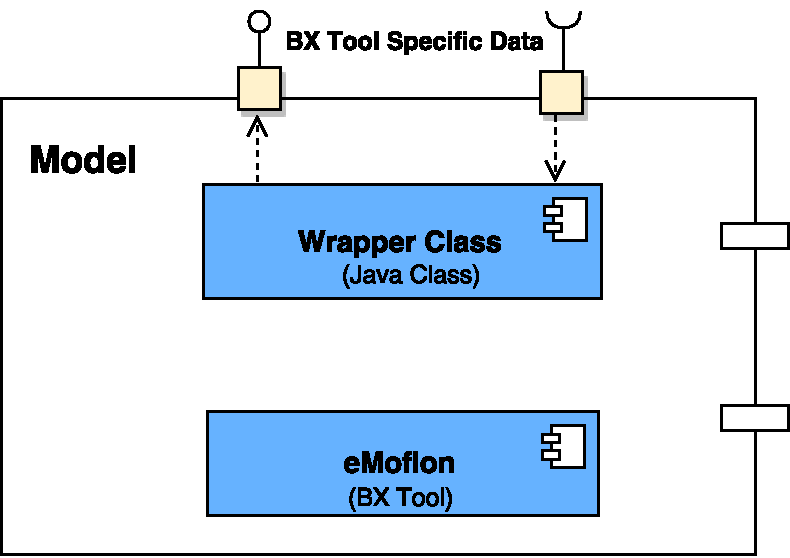
\includegraphics[width=0.8\textwidth]{figures/Component_Diagram-Model}
	\caption{Component Diagram of Model}
	\label{fig:Component_Diagram-Model}
\end{figure}

\paragraph{Sub-Components}
Figure~\ref{fig:Component_Diagram-Model} describes the architecture of the model in the form of a component diagram. In my case, the model contains two sub-components, \texttt{BX Tool Wrapper} and bx tool i.e., \texttt{eMoflon}. 

The bx tool wrapper consists of interfaces and its concrete implementation designed to access the bx tool on the top of the framework provided by the \texttt{Benchmarx}~\cite{benchmarx-reload}, a common design space to access different bx tools. With the help of this interface, the controller communicates with the bx tool i.e., eMoflon. However, the interface presented to the controller is not eMoflon specific. The bx tool wrapper for eMoflon translates this generic bx tool interface to eMoflon's interface. The eMoflon tool contains all the meta-models, state of the meta-models and the associated transformation rules.

For implementing the example \textit{Planning a Kitchen} through the \textit{eMoflon} tool, the first task was to create related models inside the tool. The bx tool will keep these models, create and manage instances of these models by applying associated transformation rules. As the example has two different views, it requires two different models in the tool as well i.e., \texttt{KitchenLanguage} to represent the symbolic view and \texttt{GridLanguage} to represent the layout view.

Figure~\ref{fig:Kitchen_MetaModel} describes the structure of the \texttt{KitchenLanguage} as a class diagram from an object-oriented point of view. It contains three classes i.e., \texttt{Kitchen}, \texttt{ItemSocket}, and \texttt{Item}. \texttt{Kitchen} class has the attributes \textit{xSize} and \textit{ySize} to describe its size and contains zero or more itemsockets. \texttt{ItemSocket} class has the attribute \textit{id} and contains exactly one item. \texttt{Item} class has the attributes \textit{xIndex} and \textit{yIndex} to describe its position. \texttt{Sink}, \texttt{Table}, and \texttt{Fridge} are different types of items.

Figure~\ref{fig:Grid_MetaModel} describes the structure of the \texttt{GridLanguage} as a class diagram from an object-oriented point of view. It contains three classes i.e., \texttt{Grid}, \texttt{Group}, and \texttt{Block}. \texttt{Grid} class has the attribute \textit{blockSize} to describe the size of each block contained inside it, contains zero or more itemsockets, and zero or more blocks. Each \texttt{Group} class occupies one or more blocks. \texttt{Block} class has the attributes \textit{xIndex} and \textit{yIndex} to describe its position and is being occupied by one group.

\begin{figure}
	\centering
	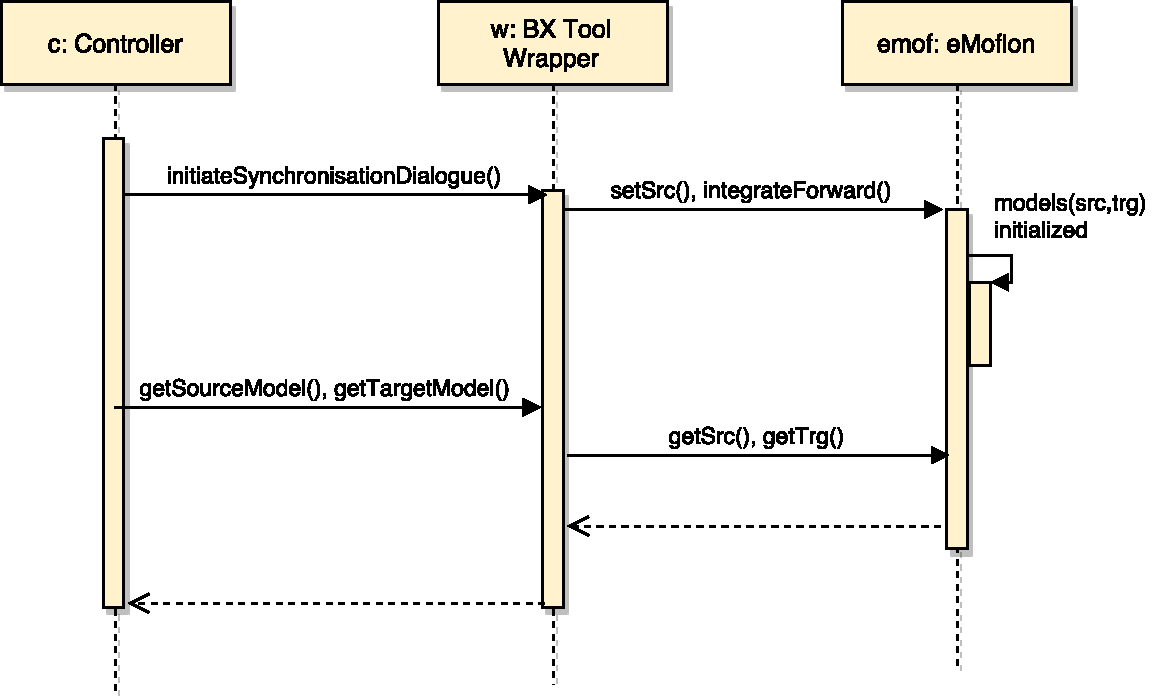
\includegraphics[width=1\textwidth]{figures/Sequence_Diagram-Model(init)}
	\caption{Sequence Diagram of Model: initialization}
	\label{fig:Sequence_Diagram-Model(init)}
\end{figure}

\begin{figure}
	\centering
	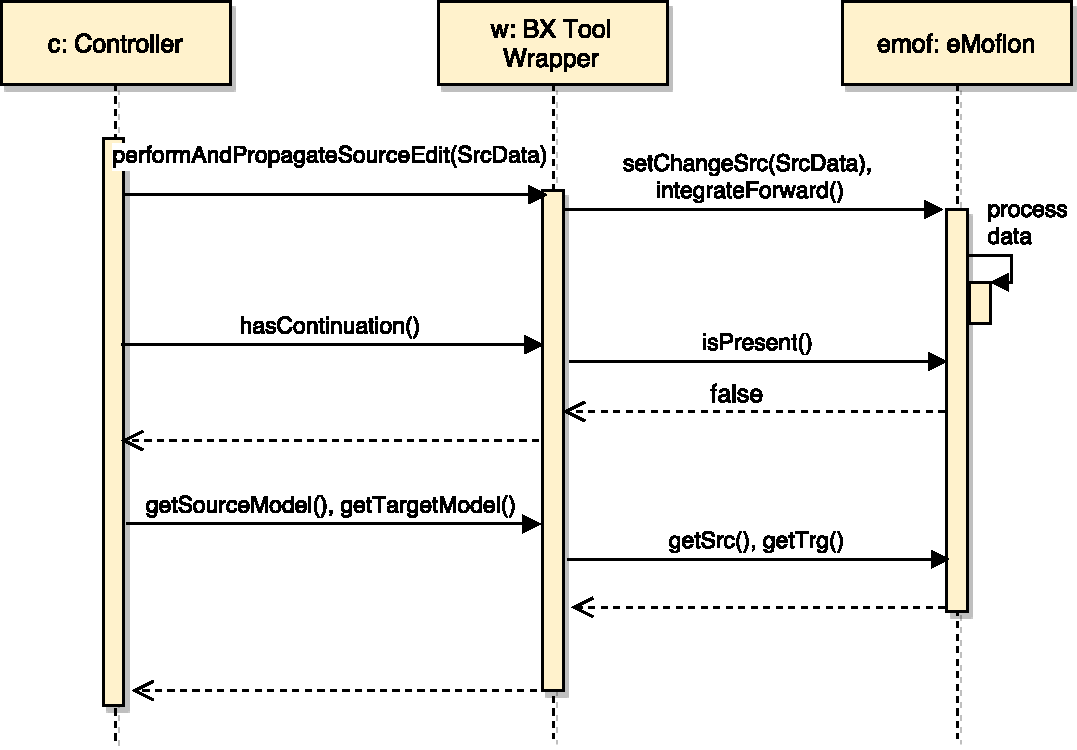
\includegraphics[width=1\textwidth]{figures/Sequence_Diagram-Model(cont-false)}
	\caption{Sequence Diagram of Model: delta propagation without continuation}
	\label{fig:Sequence_Diagram-Model(cont-false)}
\end{figure}

\begin{figure}
	\centering
	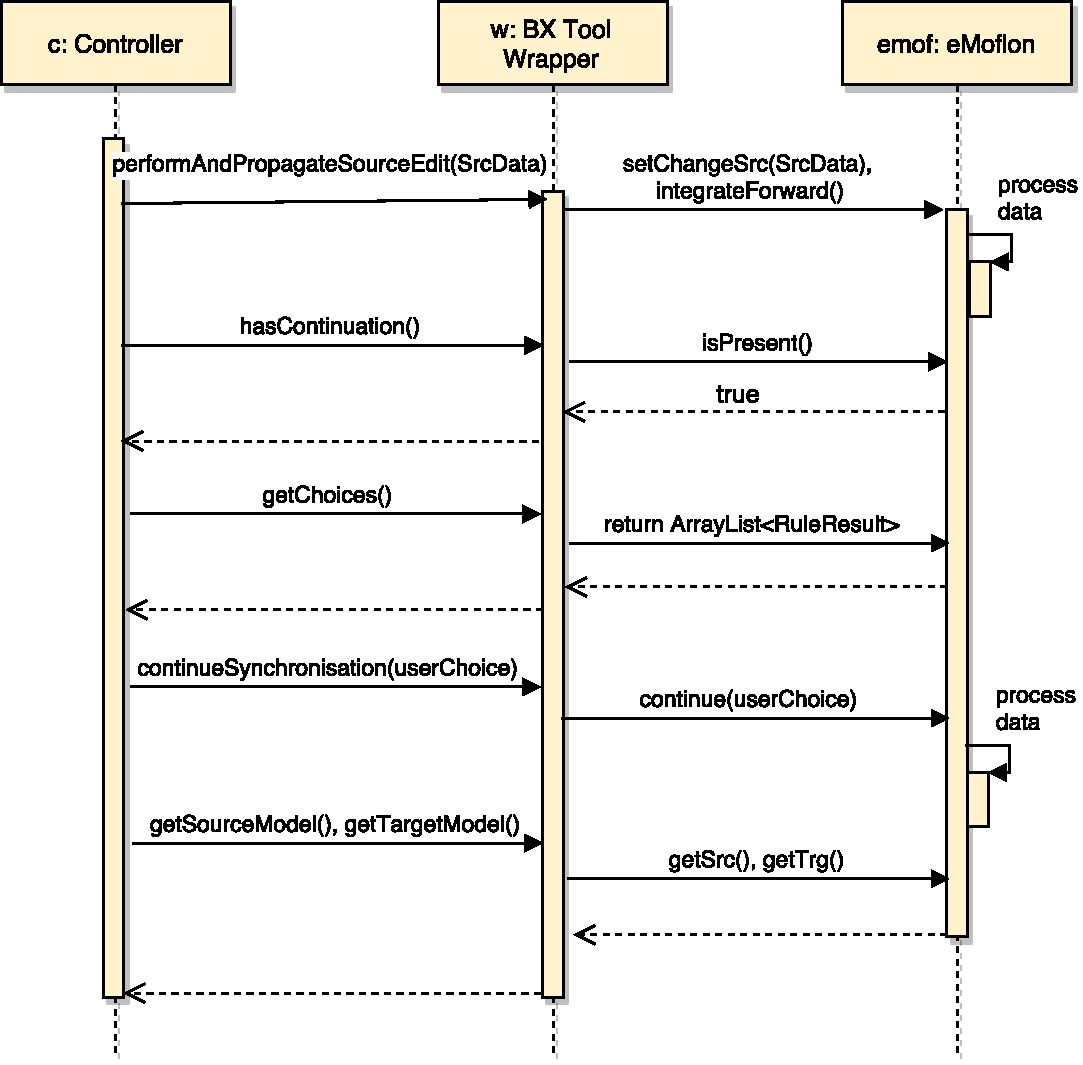
\includegraphics[width=1\textwidth]{figures/Sequence_Diagram-Model(cont-true)}
	\caption{Sequence Diagram of Model: delta propagation with continuation}
	\label{fig:Sequence_Diagram-Model(cont-true)}
\end{figure}

\paragraph{Workflow}
The sequence diagrams shown in Figure~\ref{fig:Sequence_Diagram-Model(init)}, Figure~\ref{fig:Sequence_Diagram-Model(cont-false)}, and Figure~\ref{fig:Sequence_Diagram-Model(cont-true)} illustrate the workflow of the Demon-BX tool from the point of view of the model component in different stages. As the model component only communicates with the controller, these sequence diagrams show the communication process between the controller and the sub-components of the model, \texttt{BX Tool Wrapper} and the bx tool i.e., \texttt{eMoflon}.
\begin{enumerate}
	\item {\textbf{Load}: During first time load of the application, the controller instantiates all the wrapper classes and calls the appropriate method (\texttt{initiateSynchronisationDialogue()}) to initialize the bx tool after receiving the initialization command from the view. After receiving the request, bx tool wrapper class sends the initialization signal (\texttt{setSrc(), integrateForward()}) to the bx tool i.e., eMoflon and the tool gets initialized by creating the instances of the \texttt{Source} and \texttt{Target} models. Then, the controller requests (\texttt{getSourceModel(), getTargetModel()}) for the newly generated models through the bx tool wrapper class. The wrapper class requests (\texttt{getSrc(), getTrg()}) for the tool specific models from the bx tool, receives it, and send it back to the controller. This entire process is shown in Figure~\ref{fig:Sequence_Diagram-Model(init)}.}
	
	\item {\textbf{Delta Propagation (without continuation)}: After converting the delta sent from the view into example specific data, controller calls the appropriate method (\texttt{performAndPropagateTargetEdit(SrcData)}) of the wrapper class e.g., propagate delta into source model. Accordingly, wrapper class initiate forward synchronization (\texttt{setChangeSrc(SrcData), integrateForward()}) and sends the delta to the bx tool i.e., eMoflon. Here I have described only the forward synchronization. However, the process for the backward synchronization goes analogously. The bx tool processes the delta taking into account all the associated transformation rules. During processing of the data, the controller checks if satisfiability of more than one transformation rule exists (\texttt{hasContinuation()}) for the processed data i.e., continuation. If continuation does not exist, processing is completed and the controller requests (\texttt{getSourceModel(), getTargetModel()}) for the newly generated models through the bx tool wrapper class. The wrapper class requests (\texttt{getSrc(), getTrg()}) for the tool specific models from the bx tool, receives it, and send it back to the controller. This entire process is shown in the upper part of the conditional case in Figure~\ref{fig:Sequence_Diagram-Model(cont-false)}.}
	
	\item {\textbf{Delta Propagation (with continuation)}: While the bx tool i.e., eMoflon processes the delta, the controller checks if satisfiability of more than one transformation rule exists (\texttt{hasContinuation()}) for the processed data i.e., continuation. If continuation exists, the controller requests (\texttt{getChoices()}) for the matching rules from the bx tool i.e., eMoflon through the bx tool wrapper class. The wrapper class requests, receives the matching rules from the bx tool, and send it back to the controller. On receiving the user's decision, the controller sends resume data processing signal (\texttt{continueSynchronisation(userChoice)}) along with the user's decision to the bx tool through the wrapper class. Afterward, the bx tool completes the data processing with the user's decision. Then, the controller requests (\texttt{getSourceModel(), getTargetModel()}) for the newly generated models through the bx tool wrapper class. The wrapper class requests (\texttt{getSrc(), getTrg()}) for the tool specific models from the bx tool, receives it, and send it back to the controller. This entire process is shown in the lower part of the conditional case in Figure~\ref{fig:Sequence_Diagram-Model(cont-true)}.}
\end{enumerate}

For better understanding and to avoid complexity, here I have described the delta propagation process for only a single delta. However, the user can generate multiple deltas as well. In that case, after receiving all the deltas from the view, the controller converts them to example specific data. Then, the controller handles them atomically (one by one). Hence, the above described delta propagation process (with or without continuation) is executed for each delta until the data processing is complete by the bx tool. 

\subsubsection{View}\label{subsubsec:design_view}
The view handles the graphical user interface part of the application. Hence, it contains all the graphic elements and all other HTML elements of the application. The view separates the design of the application from the logic of the application due to which the front end designer and the back end developer can work separately without thinking about the errors which could have shown up in the case of an overlapping \cite{designpattern-headfirst} \cite{mvc-arch}. The view controls how the data is being displayed, how the user interacts with it and provides ways for gathering the data from the users.

\begin{figure}[h]
	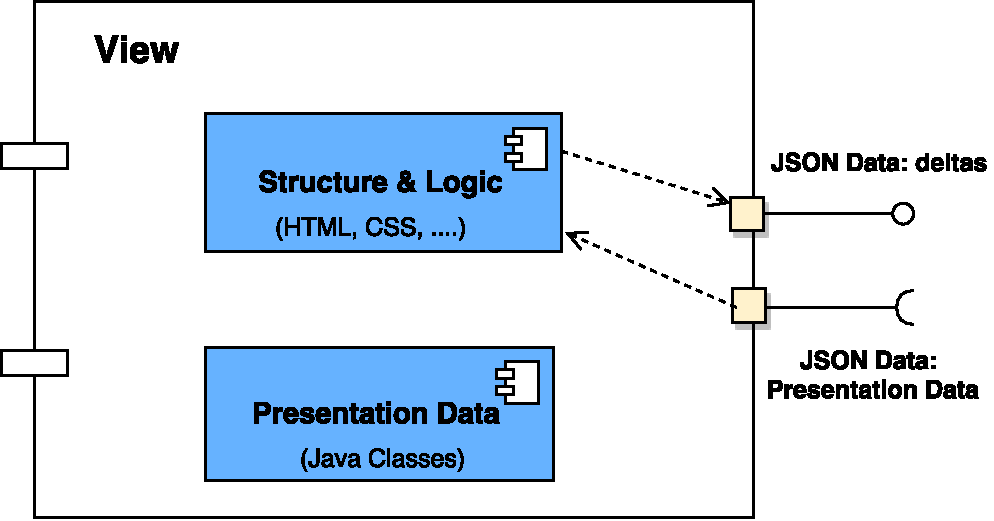
\includegraphics[width=1\textwidth]{figures/Component_Diagram-View}
	\caption{Component Diagram of View}
	\label{fig:Component_Diagram-View}
\end{figure}

\paragraph{Sub-Components}
Figure~\ref{fig:Component_Diagram-View} describes the architecture of the view in the form of a component diagram. View basically contains two sub-components, \texttt{Structure \& Logic} and \texttt{Presentation Data}. 

\texttt{Structure \& Logic} makes use of technologies like HTML, CSS, JavaScript, Jquery, and FabricJs, which combinedly create a user interface for the user to interact and the logic to handle the user actions. 

\texttt{Presentation Data} consists of Java classes created for the user interface to handle the user actions, visualize the bx tool specific models, and act a connecting bridge between them.
The view always receives the presentation data as a response from the controller in the form of JSON data and visualize them.

\begin{sidewaysfigure}
	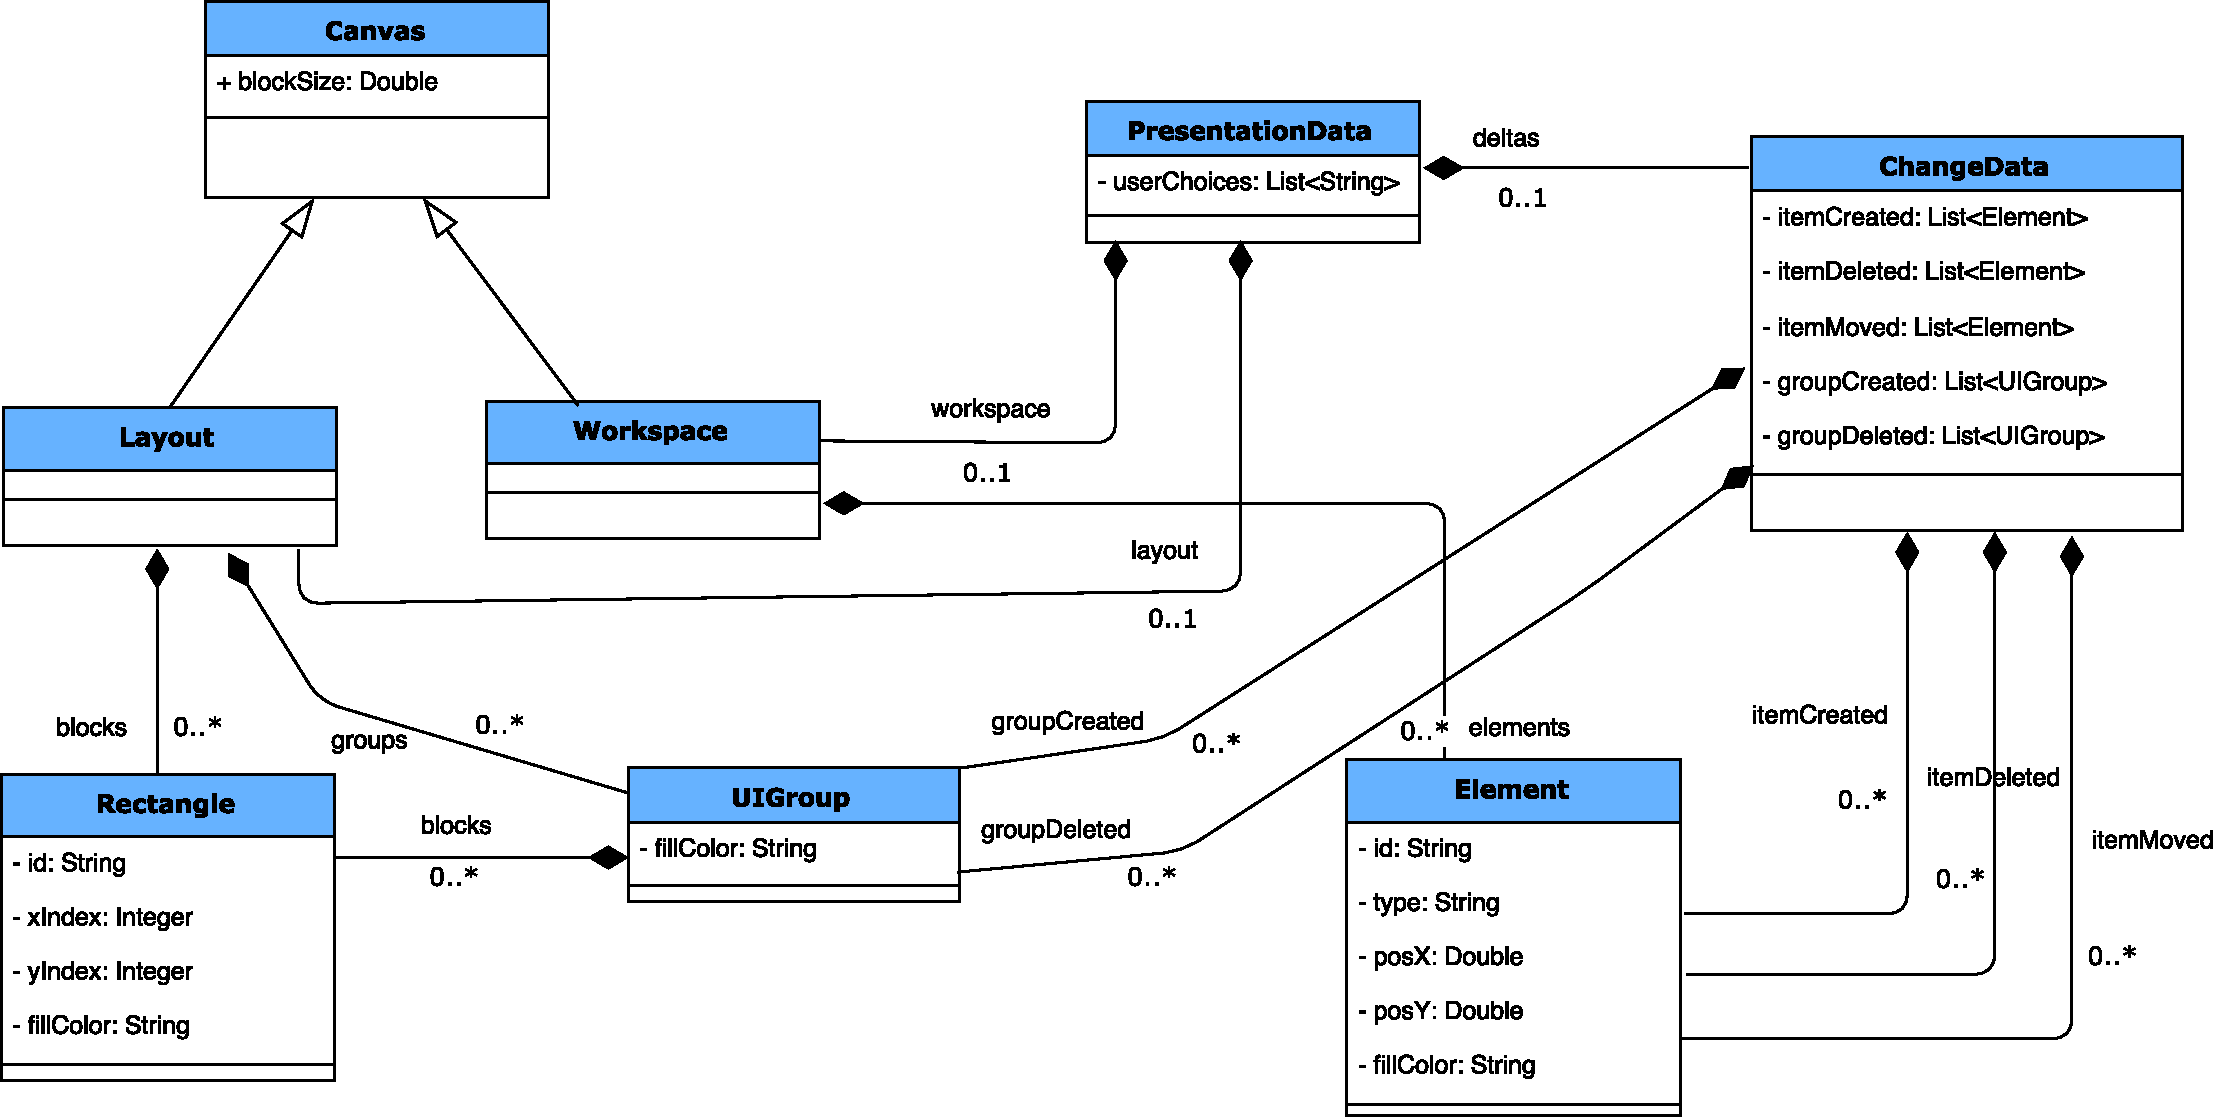
\includegraphics[width=1\textwidth]{figures/ClassDia_UI-Models}
	\caption{Class Diagram of Presentation Data}
	\label{fig:ClassDia_UI-Models}
\end{sidewaysfigure}

Figure~\ref{fig:ClassDia_UI-Models} shows the structure of the presentation data in the form of a class diagram. It consists of classes like \texttt{Canvas}, \texttt{Layout}, \texttt{Workspace}, \texttt{PresentationData}, \texttt{UIGroup}, \texttt{Element}, \texttt{Rectangle}, and \texttt{ChangeData}. \texttt{Canvas} is the parent class for \texttt{Layout} and \texttt{Workspace}. It has attributes \textit{height} and \textit{width} to describe its size representing the views. The \texttt{Workspace} represents the symbolic view in the user interface and contains zero or more objects (elements). The \texttt{Layout} represents the layout view in the user interface and contains zero or more blocks and groups. \texttt{UIGroup} has attribute \textit{fillColor} to uniquely identified as a new group on UI and contains zero or more blocks. \texttt{Rectangle} has attributes \textit{id}, \textit{xIndex}, \textit{yIndex}, and \textit{fillColor} to deal with the UI related actions. The \texttt{Element} has attributes \textit{id}, \textit{type}, \textit{xPos}, \textit{yPos}, and \textit{fillColor}. \texttt{PresentationData} is the class which carries all the information related to UI. After receiving the response from the bx tool, the controller converts the bx tool specific models into \texttt{PresentationData} and send it to view for visualization. It has an attribute userChoices and contains a layout, a workspace, and a set of deltas wrapped inside a \texttt{ChangeData} class.

While user interacts with the demonstrator, actions i.e., changes performed by the user in the UI are captured in the form of \texttt{delta}s and packaged in a \texttt{ChangeData} object. The symbolic view allows three actions i.e., creation of a new item, deletion of an item and movement of an item. Whereas, the layout view allows two actions i.e., creation of a new group and deletion of a group. Hence, \texttt{ChangeData} class tracks all of these five actions separately. \texttt{ChangeData} class shown in Figure~\ref{fig:ClassDia_UI-Models} contains itemCreated, itemDeleted and ItemMoved as a list of \texttt{Element}s to capture creation, deletion, and movement of an item respectively in the symbolic view. It also contains groupCreated and groupDeleted as a list of \texttt{UIGroup}s to capture creation and deletion of a group respectively in the layout view. Also, these \texttt{delta}s are captured atomically so that they can be executed independently by the bx tool.

\begin{figure}
	\centering
	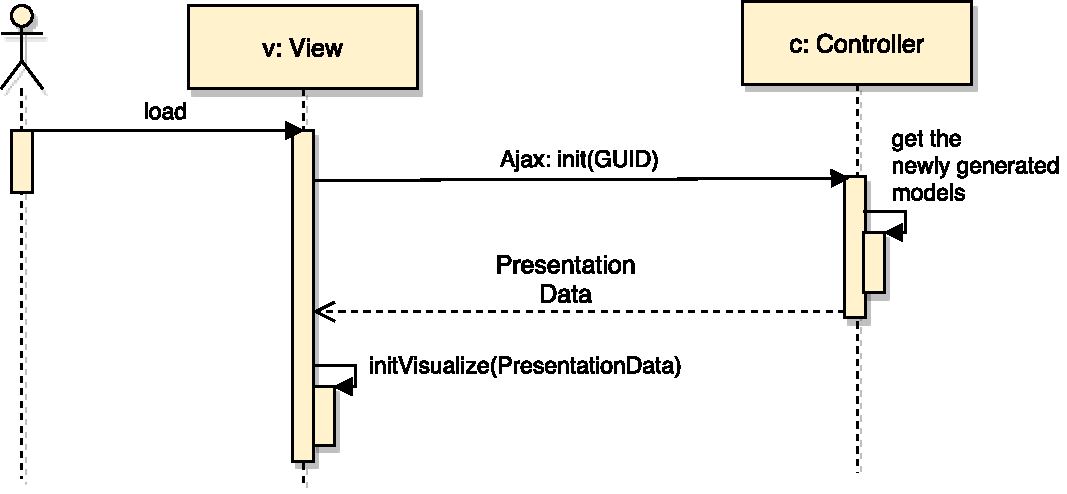
\includegraphics[width=1\textwidth]{figures/Sequence_Diagram-View(init)}
	\caption{Sequence Diagram of View: initialization}
	\label{fig:Sequence_Diagram-View(init)}
\end{figure}

\begin{figure}
	\centering
	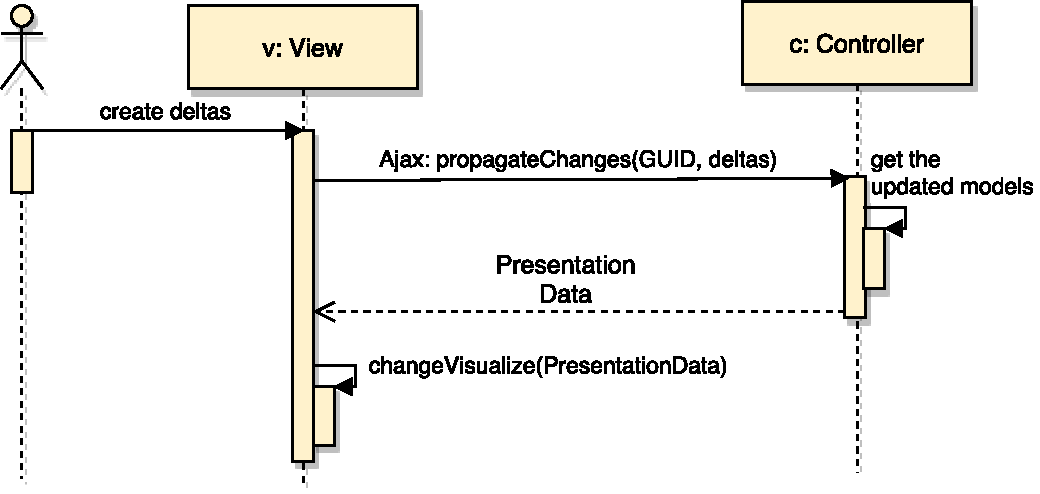
\includegraphics[width=1\textwidth]{figures/Sequence_Diagram-View(cont-false)}
	\caption{Sequence Diagram of View: delta propagation without continuation}
	\label{fig:Sequence_Diagram-View(cont-false)}
\end{figure}

\begin{figure}
	\centering
	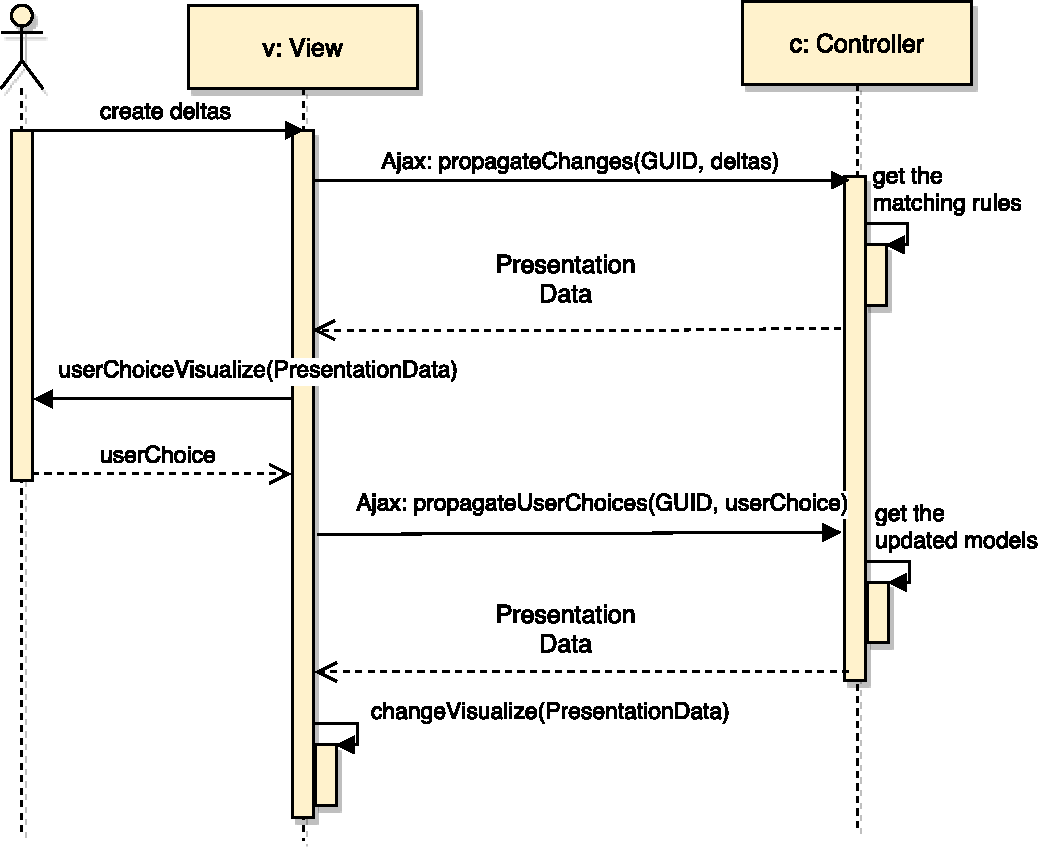
\includegraphics[width=1\textwidth]{figures/Sequence_Diagram-View(cont-true)}
	\caption{Sequence Diagram of View: delta propagation with continuation}
	\label{fig:Sequence_Diagram-View(cont-true)}
\end{figure}

\paragraph{Workflow}
The sequence diagrams shown in Figure~\ref{fig:Sequence_Diagram-View(init)}, Figure~\ref{fig:Sequence_Diagram-View(cont-false)}, and Figure~\ref{fig:Sequence_Diagram-View(cont-true)} illustrate the workflow of the Demon-BX tool from the point of view of the view component in different stages. As the view component only communicates with the controller, these sequence diagrams show the communication process between the controller and the view only.

\begin{enumerate}
	\item {\textbf{Load}: To load the application, the user enters the complete URL on a web browser. As soon as the web page is loaded, the view generates a unique user id (GUID) for the current user and sends an initialization command (\texttt{init(GUID)}) for the bx tool i.e., eMoflon along with the GUID in the form of \texttt{JSON} data to the controller wrapped inside an \texttt{Ajax} call. In return, the view gets the \texttt{PresentationData} from the controller after the initialization of the bx tool. After getting the data, the view visualizes (\texttt{changeVisualize(PresentationData)}) them in two HTML canvas elements i.e., \texttt{Layout} and \texttt{Kitchen}. This entire process is shown in Figure~\ref{fig:Sequence_Diagram-View(init)}.}
	
	\item {\textbf{Delta Propagation (without continuation)}: A user is allowed to create one or more deltas in one of the HTML canvas elements i.e., \texttt{Layout} and \texttt{Kitchen}. To propagate the deltas to the other view, the user presses the synchronization button. Then the view sends (\texttt{propagateChanges(GUID, deltas)}) all the deltas created along with the GUID generated earlier for the user in the form of \texttt{JSON} data to the controller wrapped inside an \texttt{Ajax} call. If continuation (satisfiability of more than one transformation rule) does not exist, the bx tool completes the processing and the controller gets the updated models. In return, the view gets the \texttt{PresentationData} from the controller. After getting the data, the view visualizes (\texttt{changeVisualize(PresentationData)}) them in two HTML canvas elements i.e., \texttt{Layout} and \texttt{Kitchen}. This entire process is shown in Figure~\ref{fig:Sequence_Diagram-View(cont-false)}.}
	
	\item {\textbf{Delta Propagation (with continuation)}: During processing of the data, If continuation (satisfiability of more than one transformation rule) exists, the controller gets the matching rules from the bx tool. In return, the view gets the \texttt{PresentationData} with user choices from the controller. After getting the data, the view 
	prompts (\texttt{userChoiceVisualize(PresentationData)}) the choices to the user and gets a decision in return. 
	View sends (\texttt{propagateUserChoices(GUID, userChoice)}) the user's choice along with the GUID generated earlier for the user in the form of \texttt{JSON} data to the controller wrapped inside an \texttt{Ajax} call. Then, the bx tool completes the processing and controller gets the updated models. In return, the view gets the \texttt{PresentationData} from the controller. After getting the data, the view visualizes (\texttt{changeVisualize(PresentationData)}) them in two HTML canvas elements i.e., \texttt{Layout} and \texttt{Kitchen}. This entire process is shown in Figure~\ref{fig:Sequence_Diagram-View(cont-true)}.}
\end{enumerate}

\paragraph{External Design}
For the visualization of the chosen example \textit{Planning a Kitchen} as explained in Section \ref{subsec:exampleforimplementation}, the first task was to design the layout view and the symbolic view along with its functionalities. However, the user interface is independent of any specific example and can be extended to implement a family of (similar) examples.

Both the views represent a workspace area and its certain behavior. The symbolic view has more functionalities and flexibility in usage than the layout view. As both the views are independent of each other and resonates a confined area in which certain task related to animation/graphics has to be performed, I chose \textit{Canvas} \cite{canvas} HTML element as a container for my views. \textit{Canvas} was the best fit for my views as it provides great support and application for creating animation and drawing graphics on the web.

\begin{figure}
	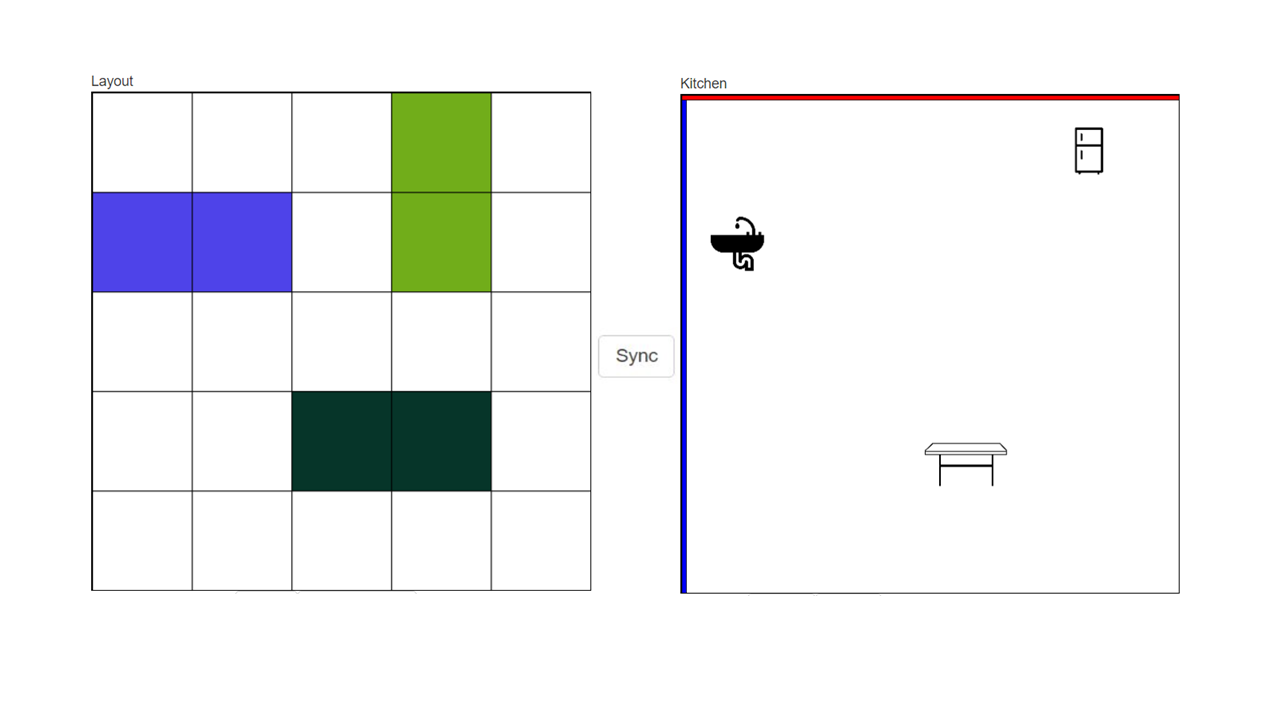
\includegraphics[width=1\textwidth]{figures/Layout_Kitchen}
	\caption{Layout and Kitchen}
	\label{fig:Layout_Kitchen}
\end{figure}

For the symbolic view, I kept the \textit{Canvas} clean to represent an empty space where addition and manipulation of different objects can be done. As the user interface is meant to be example independent, the four sides of the \textit{Canvas} are "special" and can be interpreted in some way for a certain example to make things more interesting. For example, for the implementation of the example \textit{Planning a Kitchen}, the four sides represent four walls of a kitchen space inside which different kitchen objects such as sink, table, fridge etc. can be added. Also, to make the kitchen space more realistic, I have even added {\color{blue} water outlets} on the western wall and {\color{red} electrical fittings} on the northern wall so that the user can relate to it. For layout view, I have filled the \textit{Canvas} with grids/blocks. The layout view represents exact workspace space as shown in the symbolic view but, divided into blocks which restrict certain flexibility and functionality. Figure~\ref{fig:Layout_Kitchen} shows a sample of the symbolic view (Kitchen) and layout view (Layout).

Next step was to handle the user interactions in the process of performing various task on both the views. In web development, javascript is the most used language for handling the user interactions and programming the behavior of web pages \cite{javascript}. Hence, I have analyzed a few canvas libraries available in market e.g., Fabric.js \cite{fabricjs}, Processing.js \cite{processingjs}, Pixi.js \cite{pixijs}  by working on a few Proof of Concepts (PoC). The main idea was to check the feasibility and support for interactivity to perform different user defined tasks on the \textit{Canvas}. Finally, I chose Fabric.js as my javascript library for handling the user interactions because of below factors \cite{fabricjs}:
\begin{itemize}
	\item {It is good at displaying a large number of objects on the canvas.}
	\item {It handles object manipulation such as, moving, rotating, resizing for any kind of object.}
	\item {It has a great support for rendering and displaying object of any kind.}
\end{itemize}

\paragraph{Internal Design}
Second task in the process of visualization was defining the user actions with respect to both the views, capturing them, and displaying the views after transformation is done.

In the symbolic view, a user can perform addition, removal, and movement of any objects. A new object can be added and an already existing object can be moved or removed within the empty space available with the different mouse events. Every object is tracked on the basis of its position in the view and every change i.e., creation, deletion or movement of objects is captured inside a \texttt{delta} by the symbolic view and send it to the controller for further processing. For example, for the implementation of the example \textit{Planning a Kitchen}, a user can create, delete or move different kitchen objects such as sink, table, fridge etc. Also, to make the example more realistic, I have used similar images of the kitchen objects as shown in the right side canvas (kitchen) in Figure~\ref{fig:Layout_Kitchen}. 

As the layout view is divided into blocks and offers fewer functionalities than the symbolic view, a user can perform only addition and removal of the objects. Hence, each object is represented in the form of a group, combining any number of block(s) arranged in vertical or in horizontal direction filled with a unique color everytime a new object is added. Every group is tracked on the basis of the block's position that it is consist of along with its color and every change i.e., addition or removal is captured inside a \texttt{delta} by the layout view and sent to the controller for further processing. For example, for the implementation of the example \textit{Planning a Kitchen}, the sink is represented by two horizontal blocks attached to one another and filled with {\color{blue} blue} color as shown in the left side canvas (layout) in Figure~\ref{fig:Layout_Kitchen}. 

After the changes are done on either view, to see the effect on the other, the user can click on the synchronization button and both the views will be updated.
 
\subsubsection{Controller}\label{subsubsec:design_controller}
The controller is mainly responsible for event/action handling and manages the relationship between a view and a model \cite{mdd-webwithmvc}. These actions are triggered while a user interacts with the application on a web browser. It accepts the user requests, interacts with the model, and generates the view from the response.

\begin{figure}[h]
	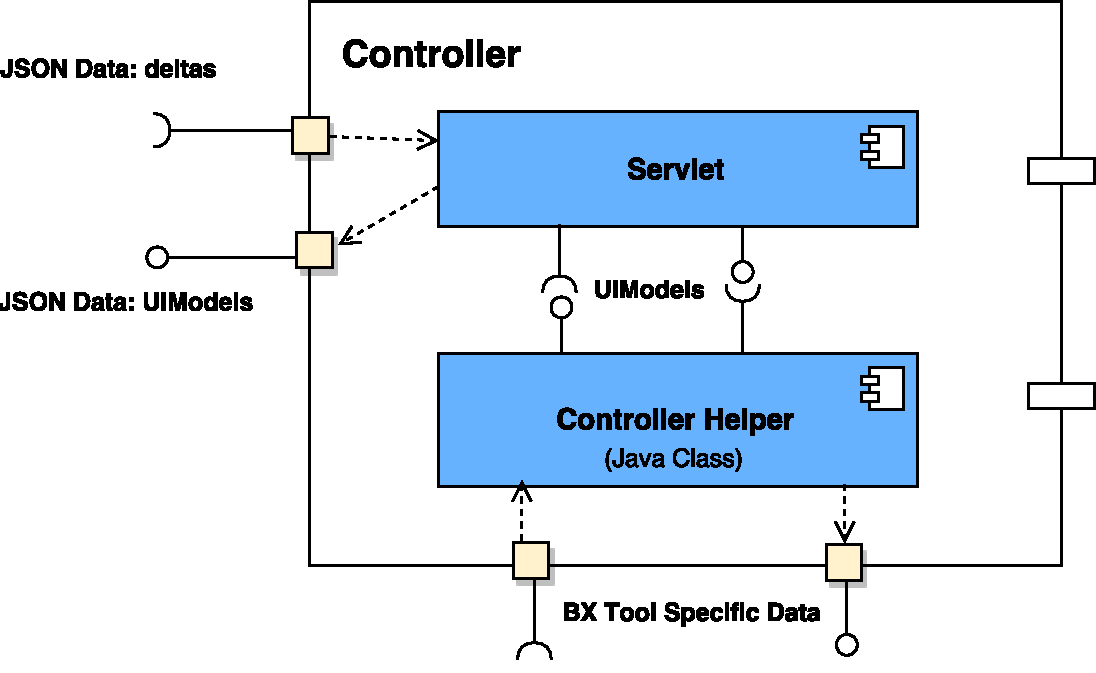
\includegraphics[width=1\textwidth]{figures/Component_Diagram-Controller}
	\caption{Component Diagram of Controller}
	\label{fig:Component_Diagram-Controller}
\end{figure}

\paragraph{Sub-Components}
Figure~\ref{fig:Component_Diagram-Controller} describes the architecture of the controller in the form of a component diagram. In my case, controller consists of two sub-components, \texttt{Servlet} and an \texttt{Adapter}.

Servlet is a technology which provides a component-based, platform-independent method for building Web-based applications \cite{servlet}. Servlet is built on Java platform to extend the capabilities of a web server which makes it robust and scalable. It resides inside a web server to generate dynamic content.

Servlet is capable of handling all kinds of client-server protocol but popularly and mostly used with the HTTP, the HyperText Transfer Protocol. A web container is essentially required to run a servlet. A web container is a component of the web server that interacts with the servlets and manages the lifecycle of servlets. In my case, I am using \textit{Apache Tomcat} as my web container. Please refer Appendix for more information about servlet lifecycle.

In my application, the servlet is strongly coupled with an adapter i.e., a Java class. The adapter is responsible for the conversion between UI data and bx tool specific data.

\begin{figure}
	\centering
	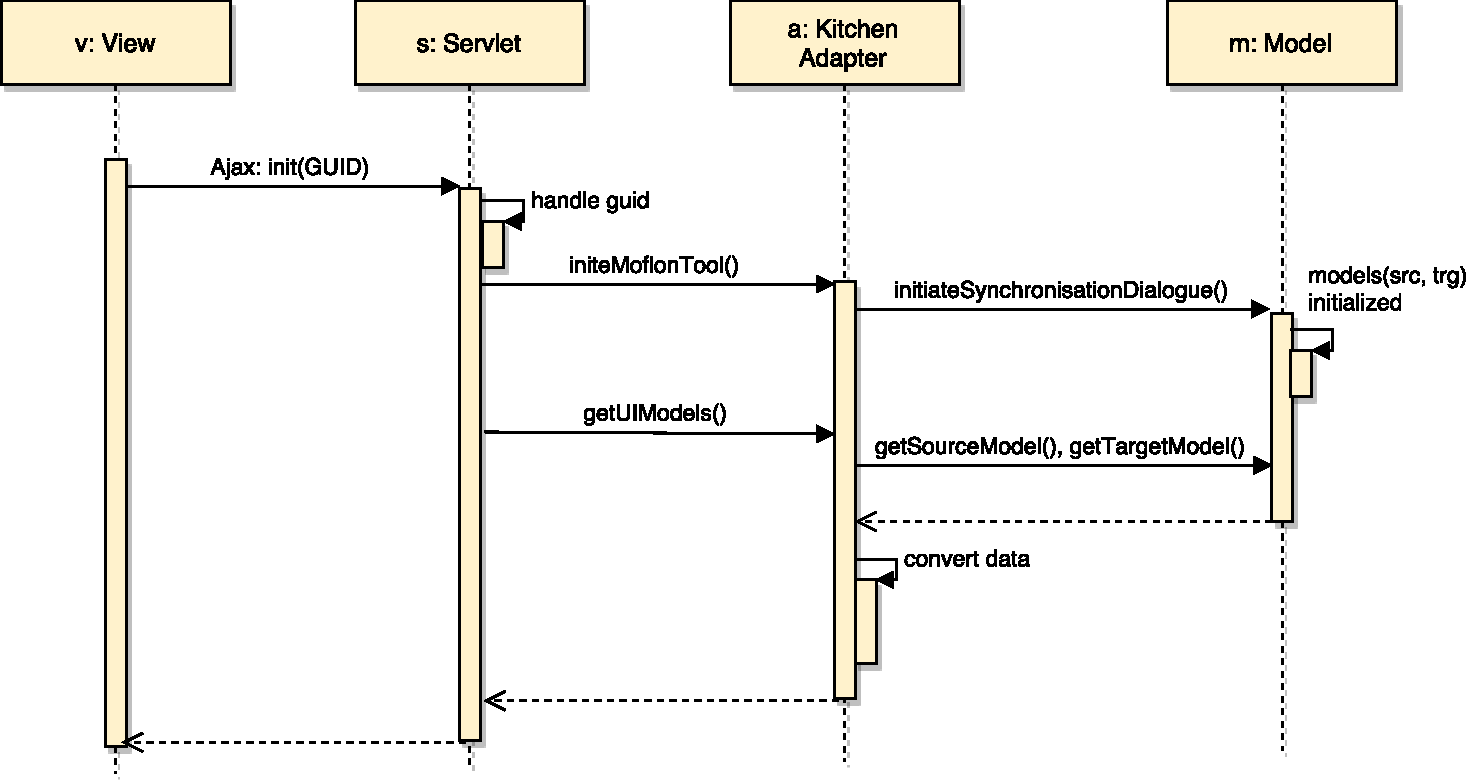
\includegraphics[width=1\textwidth]{figures/Sequence_Diagram-Controller(init)}
	\caption{Sequence Diagram of Controller: initialization}
	\label{fig:Sequence_Diagram-Controller(init)}
\end{figure}

\begin{figure}
	\centering
	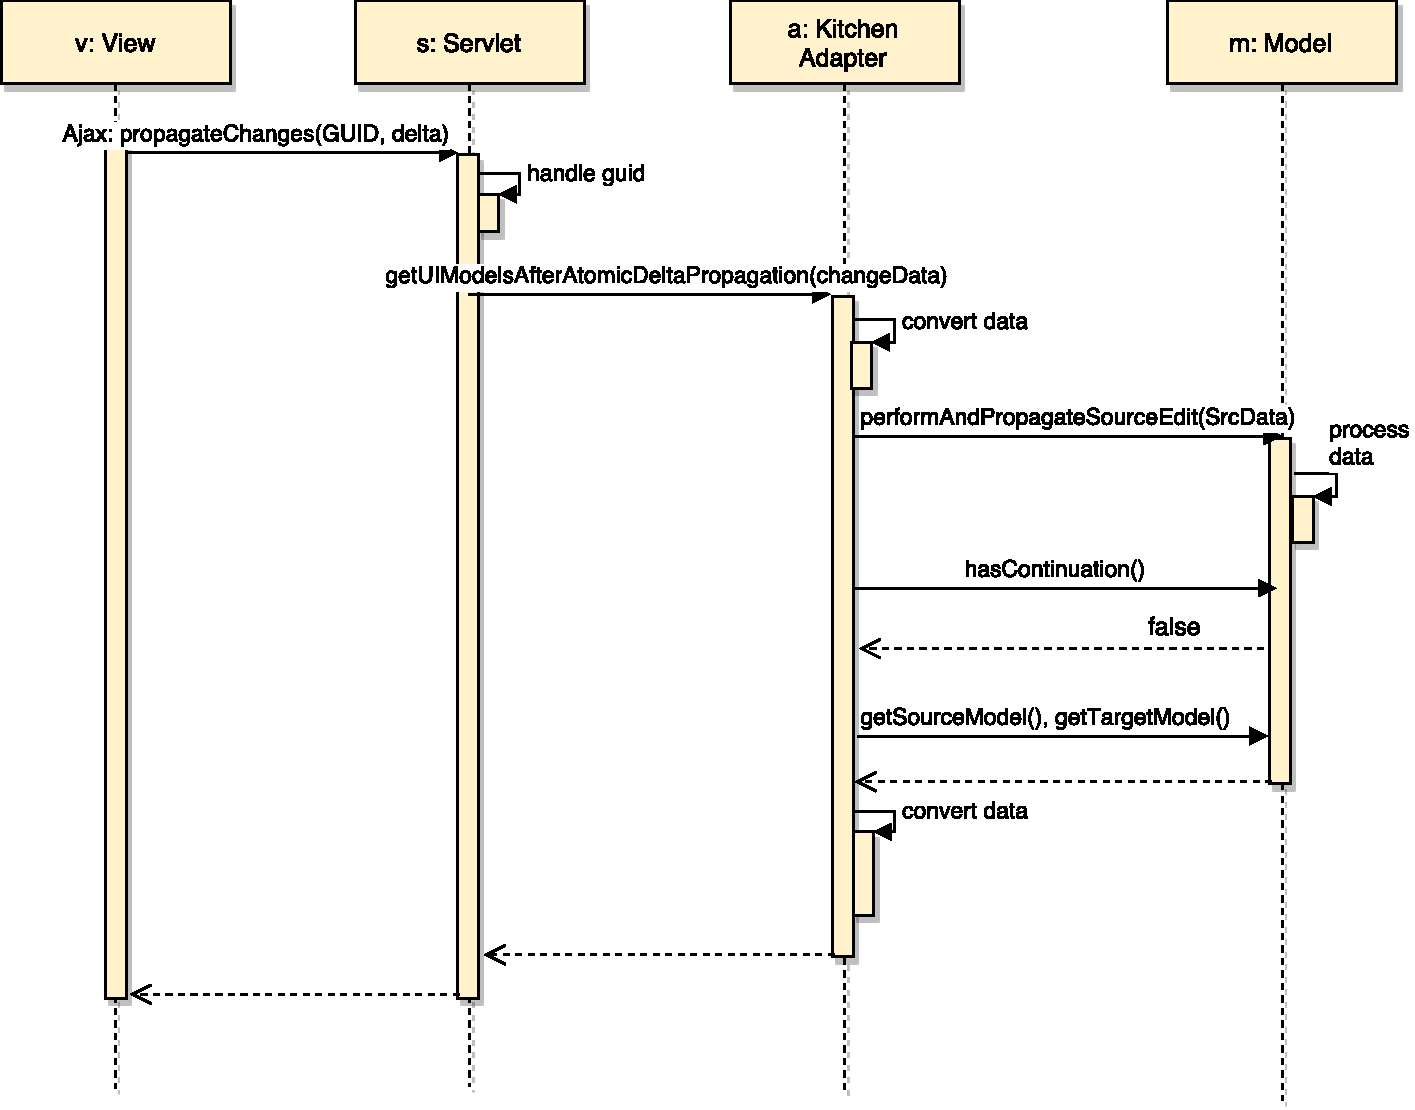
\includegraphics[width=1\textwidth]{figures/Sequence_Diagram-Controller(cont-false)}
	\caption{Sequence Diagram of Controller: delta propagation without continuation}
	\label{fig:Sequence_Diagram-Controller(cont-false)}
\end{figure}

\begin{figure}
	\centering
	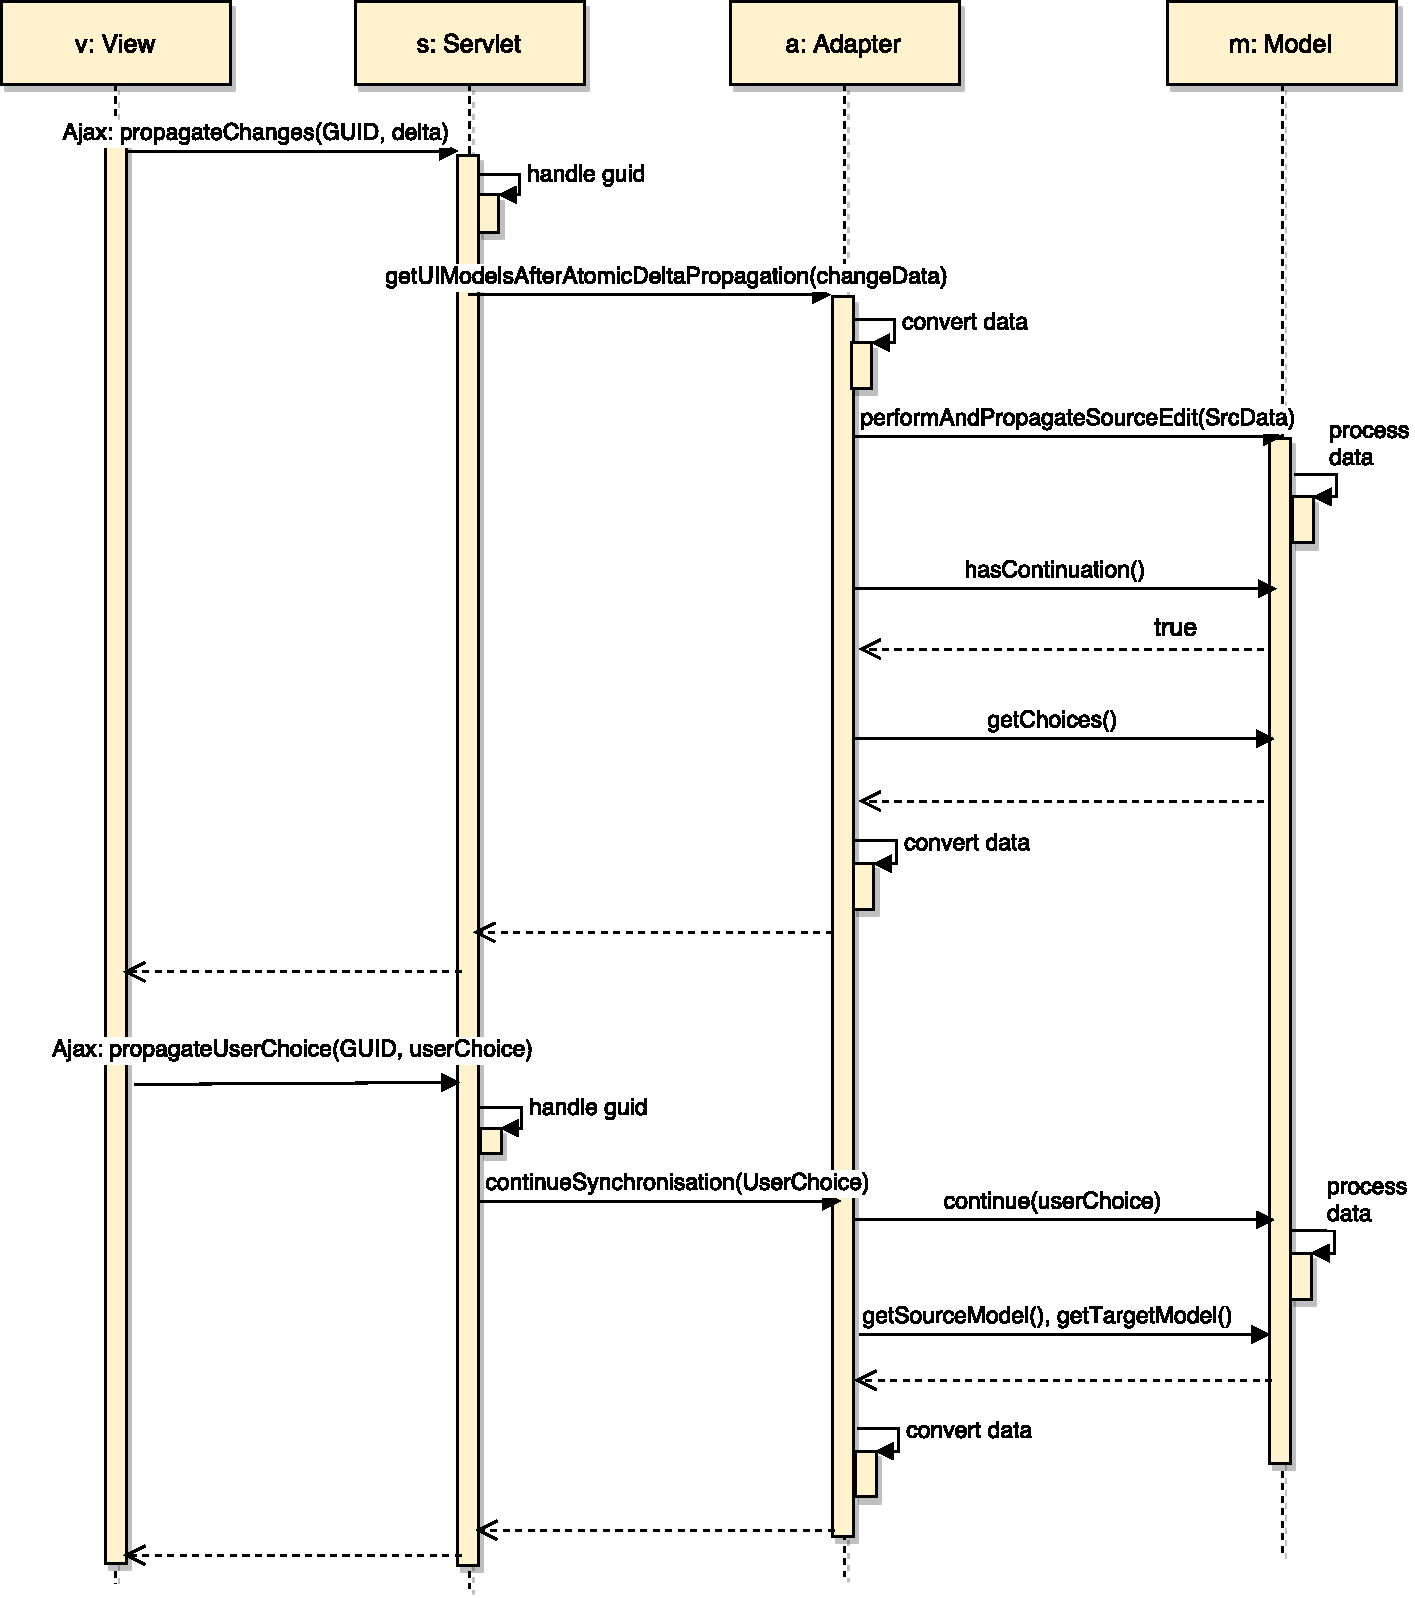
\includegraphics[width=1\textwidth]{figures/Sequence_Diagram-Controller(cont-true)}
	\caption{Sequence Diagram of Controller: delta propagation with continuation}
	\label{fig:Sequence_Diagram-Controller(cont-true)}
\end{figure}

\paragraph{Workflow}
Figure~\ref{fig:Sequence_Diagram-Controller(init)}, 
Figure~\ref{fig:Sequence_Diagram-Controller(cont-false)},
and Figure~\ref{fig:Sequence_Diagram-Controller(cont-true)} illustrate the workflow of the Demon-BX tool from the point of view of the controller component in different stages. As the controller component communicates with both the view and model, these sequence diagrams show the communication process between the view, model and the sub-components of the controller, \texttt{Servlet} and the \texttt{Adapter}.

\begin{enumerate}
	\item {\textbf{Load}: During first time load of the application, the servlet receives an initialization command (\texttt{init(GUID)}) from the view along with the newly generated GUID for the user in the form of \texttt{JSON} data wrapped inside an \texttt{Ajax} call. After receiving the request, the servlet creates a new instance of the adapter and stores the GUID. Then, the servlet forwards the initialization request (\texttt{initeMoflonTool()}) to the adapter. The adapter instantiates the bx tool i.e., eMoflon tool (\texttt{initiateSynchronisationDialogue()}) and the tool gets initialized by creating the instances of the \texttt{Source} and \texttt{Target} models. Afterward, servlet requests 
	(\texttt{getUImodels()}) for the newly generated models through the adapter. The adapter requests (\texttt{getSourceModel(), getTargetModel()}) for the example specific models from the model, receives it, converts it to the UI specific data, and send it back to the servlet. After receiving the response, the servlet forwards it to the view for visualization. This entire process is shown in Figure~\ref{fig:Sequence_Diagram-Controller(init)}.}
		
	\item {\textbf{Delta Propagation (without continuation)}: After the synchronization button is pressed, view sends (\texttt{propagateChanges(GUID, delta)}) the delta created along with the GUID generated earlier for the user in the form of \texttt{JSON} data to the servlet wrapped inside an \texttt{Ajax} call. After receiving the request from the view, the servlet handles the GUID (checks its existence) and forwards (\texttt{getUIModelsAfterAtomicDeltaPropagation(changeData)}) the delta wrapped inside a \texttt{ChangeData} class to the adapter. After converting the delta into example specific data, adapter calls the appropriate method (\texttt{performAndPropagateSourceEdit(SrcData)}) and sends the delta to the bx tool i.e., eMoflon. Here I have described only the forward synchronization. However, the process for the backward synchronization goes analogously. The bx tool processes the delta taking into account all the associated transformation rules. During processing of the data, adapter checks if satisfiability of more than one transformation rule exists (\texttt{hasContinuation()}) for the processed data i.e., continuation. If continuation does not exist, processing is completed by the bx tool. Then the adapter requests (\texttt{getSourceModel(), getTargetModel()}) for the updated example specific models from the model, receives it, converts it to the UI specific data, and send it back to the servlet. After receiving the response, the servlet forwards it to the view for visualization. This entire process is shown in Figure~\ref{fig:Sequence_Diagram-Controller(cont-false)}.}
	
	\item {\textbf{Delta Propagation (with continuation)}: During processing of the data, If continuation (satisfiability of more than one transformation rule) exists, adapter requests for the matching rules (\texttt{getChoices()}) from the bx tool i.e., eMoflon, converts them into the UI specific data, and send it back to the servlet. The servlet forwards it to the view for visualization. After getting the user's choice, view sends (\texttt{propagateUserChoice(GUID, userChoice)}) it along with the GUID generated earlier for the user in the form of \texttt{JSON} data to the servlet wrapped inside an \texttt{Ajax} call. After receiving the request from the view, the servlet handles the GUID (checks its existence) and forwards (\texttt{continueSynchronisation(userChoice)}) the user's choice to the adapter. The adapter forwards it to the bx tool for further processing. Then the adapter requests (\texttt{getSourceModel(), getTargetModel()}) for the updated example specific models from the model, receives it, converts it to the UI specific data, and send it back to the servlet. After receiving the response, the servlet forwards it to the view for visualization. This entire process is shown in Figure~\ref{fig:Sequence_Diagram-Controller(cont-true)}.}
\end{enumerate}

For better understanding and to avoid complexity, here I have described the delta propagation process for only a single delta. However, the user can generate multiple deltas as well. In that case, after receiving all the deltas from the view, the controller converts them to example specific data. Then, the controller handles them atomically (one by one). Hence, the above described delta propagation process (with or without continuation) is executed for each delta until the data processing is complete by the bx tool.

\subsection{Challenges}\label{subsec:designchallenges}
During the entire designing and implementation process as explained in previous sections of this chapter, I came across a few challenges. This section describes them in detail. 

\paragraph{UI interaction and capturing deltas}
From UI design and interaction point of view, after designing the views i.e., an empty canvas(Kitchen) to represent the symbolic view and a canvas filled with blocks(Layout) to represent the layout view, the first challenge was conceptualizing \texttt{delta}s and capturing them. 

\begin{figure}[h]
	\includegraphics[width=1\textwidth]{figures/layout}
	\caption{Layout View}
	\label{fig:Layout}
\end{figure}

As mentioned earlier, the symbolic view has more functionalities than the layout view in example \textit{Planning a Kitchen}. Firstly, I fixed the deltas that can be performed on either view. For example, three types of changes are allowed in the kitchen i.e., creation of a new item, deletion of an item, and movement of an item. Whereas, two types of changes are allowed in the layout i.e., creation of a new group and deletion of a group. Implementing the user interactions in the kitchen was relatively easy as the user has to deal with the creation, deletion, and movement of objects with actions such as mouse movements and button clicks. But, the real challenge was to handle the user interactions in the block structure of the layout. After having a few discussions, I decided to go ahead with colored blocks to show the occupancy of groups in the layout. Each group will be shown with a set of unique colored blocks. A user can generate different colors by multiple mouse clicks to fill an empty/non-occupied block while creating a new group and same colored blocks will be considered as one group. For deletion of a group, a user can click on any one of the same colored blocks (blocks belong to the same group) and blur its color. 

\textit{Example:} Figure~\ref{fig:Layout} shows a sample of the layout with a different set of groups filled with different colors. The layout contains three groups separated by three unique colors i.e., two horizontally adjacent blocks on the western wall with {\color{blue} blue} color, two vertically adjacent blocks on the northern wall with {\color{darkgreen} dark green} color, and two horizontal adjacent blocks in the middle of the layout with {\color{darkgray} dark gray} color.

\paragraph{Compressing related deltas}
Along with creating deltas, another challenge was to compressing different deltas (in some cases) into one in the process of capturing. Capturing every change that occurs on the views and sending them to the bx tool for processing is error-prone, complex, and sometimes even not required for the tool to handle. For example, creating an item in the kitchen, then deleting it and sending both of the changes to the bx tool do not make sense as the item does not exist anymore. Hence, rather capturing every change that occurs on the views, I have implemented a few rules while capturing them. The handling of a single delta is clear. But, the interesting part is rules for how to compress two deltas into one in some cases. All possible combinations are described in Figure~\ref{fig:seriesofdeltas}.

\begin{figure}[h]
	\centering
	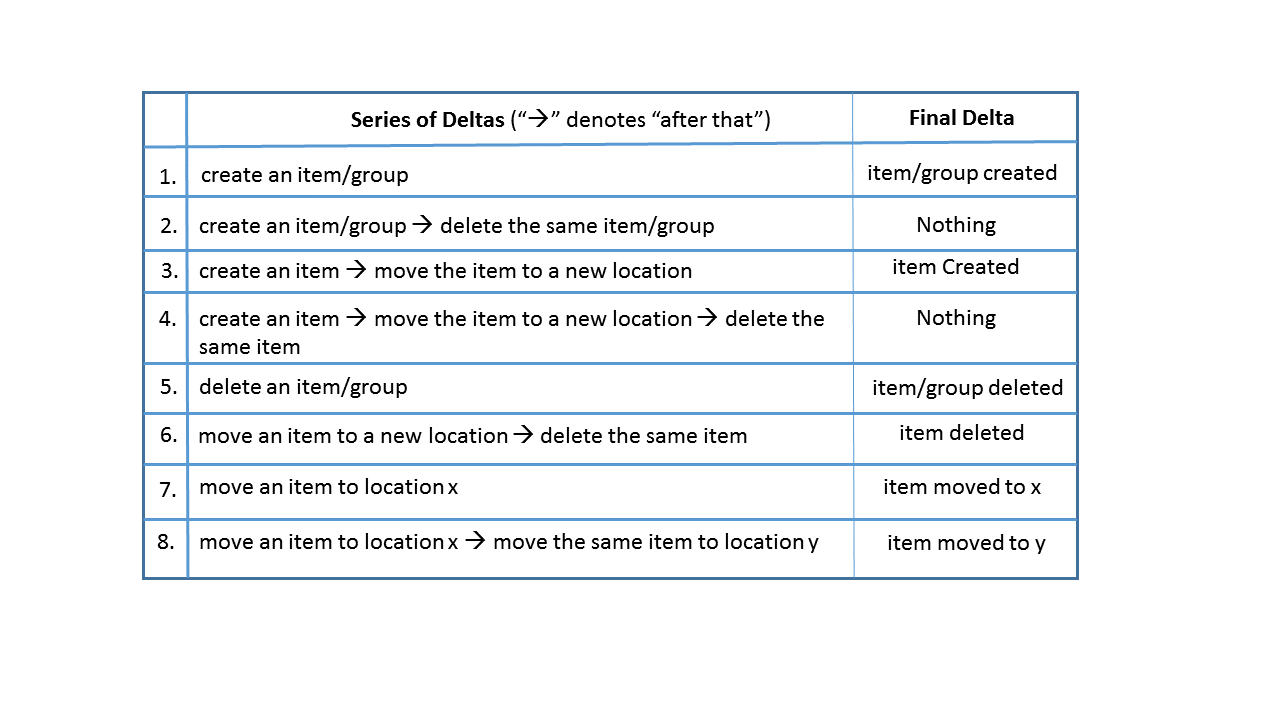
\includegraphics[width=1\textwidth]{figures/seriesofdeltas}
	\caption{Rules for compressing deltas}
	\label{fig:seriesofdeltas}
\end{figure}

\textit{Example:} A user creates a table in the kitchen and then move it to a new location. In this situation, instead of creating two different deltas, I capture only one i.e., item created at a new location. Because creating a new item and then moving it to a new location is equivalent to creating a new item at the new location.

\paragraph{Handling failed deltas}
Another challenge was to handle the rejected/failed deltas during and after the processing by the eMoflon tool. The problem was when a series of deltas are given to the eMoflon tool for processing, not all of them are accepted and processed but some of them are rejected as well according to the associated transformation rules. So, if the eMoflon tool is fed with a series of deltas at one go, it will not process the remaining deltas after encountering the first invalid delta even if all or some of the remaining deltas are valid. Also, after processing only the accepted deltas will be contained in the updated models and it will not be possible to track the rejected deltas. 

To solve this problem, I decided to implement \textit{atomic delta} method. In this method, deltas are given to the eMoflon tool for processing one after another from the pool of the collected deltas from \texttt{Controller}. If any of the deltas is rejected during processing, eMoflon sends it to the \texttt{Controller}, restores the state of the models to the previous consistent state, and resume processing the remaining deltas. After the completion of processing, \texttt{Controller} gathers all the \textit{failed delta}s as \texttt{deltas} bundled inside the \texttt{PresentationData} class as shown in Figure~\ref{fig:ClassDia_UI-Models} and sends it to the view for visualization. 

\textit{Example:} A user creates two deltas in the kitchen i.e., moving an already existing fridge away from the wall with electrical fittings (invalid delta) and creating a new sink close to the wall with water outlet (valid delta). After pressing the synchronization button, both the deltas are sent to the eMoflon tool but fed one by one. As the movement of the fridge is an invalid delta, the tool rejects the delta, sends it to the controller, restores the state of the models to the previous consistent state, and resume processing the remaining deltas. Then, the processing of the delta for the creation of a new sink will be accepted by the tool and models will be updated as it is a valid delta.

\paragraph{Processing deltas in correct order}
One of the challenges during the implementation phase was in which order the deltas are supposed to be fed to the eMoflon tool for processing. It is important to consider the correct order of processing the deltas as a wrong order create conflict while processing. For example, a user deletes an item x from a location and then move another item y to the same location. While processing, delta for movement will be rejected by the eMoflon tool if it is processed first. Because the tool will not move the item y to the location where item x is still present. So the correct order is deletion then movement and creation at the end. This is because of the fact that creation of a new item depends on the movement and deletion of an already existing item and movement of an item depends on the deletion of an already existing item as shown in Figure~\ref{fig:State_Dependency}. Hence, in my implementation, all the deltas related to deletion are processed first. Then, all the deltas related to movement are processed and at the end, all the deltas related to creation are processed.  

\begin{figure}
	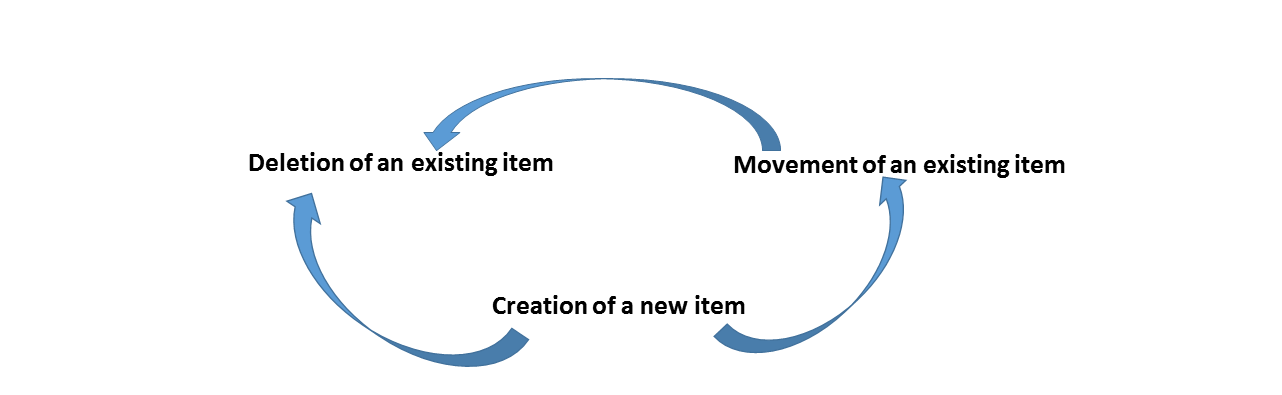
\includegraphics[width=1\textwidth]{figures/State_Dependency}
	\caption{Dependency of states with each other}
	\label{fig:State_Dependency}
\end{figure}

\textit{Example:} A user creates two deltas in the kitchen i.e., deleting an already existing sink from the location "x" (valid delta) and moving an already existing table to the location "x" (valid delta). After pressing the synchronization button, both the deltas are sent to the eMoflon tool but fed one by one in the order deletion of the sink then the movement of the table. Processing of the deletion of the sink will be accepted by the tool and models will be updated as it is a valid delta. Then, the processing of movement of the table will also be accepted by the tool and models will be updated as it is a valid delta. But, the important part is if the processing of the delta for movement of the table to the location "x" was processed first, then eMoflon would have rejected it. Because the tool will not move the table to the location "x" where a sink is still present.

\paragraph{Handling multiple users accessing the application}
Another challenge that I faced during the implementation of the servlet was handling multiple user's requests accessing the application at the same time. The problem was to maintain different states of the bx tool specific models for different users. 

\begin{figure}
	\centering
	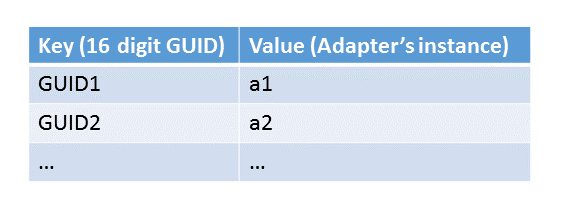
\includegraphics[width=1\textwidth]{figures/Keyvalue_map}
	\caption{Key-Value map for storing GUID}
	\label{fig:Keyvalue_map}
\end{figure}

I solved this problem by generating a unique user id (GUID) for a user on the first time load of the application and associating all the further requests from that user with the specific GUID generated earlier till the browser is closed. On the first time load of the application, view generates a random sixteen digit unique user id (GUID) for the current user and sends it with the initialization request in the form of \texttt{JSON} data to the servlet wrapped inside an \texttt{Ajax} call. As the GUID contains sixteen digits generated randomly from system's time stamp, it is almost impossible that two users will have the same GUID. After receiving the request, the servlet creates a new instance of the adapter class and stores the GUID pointing to the newly created instance of the adapter inside a \texttt{key-value map} as shown in Figure. Then, the servlet forwards the initialization request to the newly created instance of the adapter class. As explained earlier in Section~\ref{subsubsec:design_controller}, the adapter initializes and communicates with the model and hence each instance of the adapter class is associated with a unique instance of the bx tool i.e., eMoflon. Hence, storing a GUID pointing to an instance of the adapter class actually maintains a link between a user and a specific instance of the bx tool i.e., instances of the bx tool specific models. Afterward, view always sends any request to the servlet along with the GUID generated earlier for the user. After receiving the request from the view, the servlet extracts the GUID and checks its existence inside the  key-value map. If the GUID exists, the servlet forwards the request to the corresponding adapter's instance. Finally, when the user closes the browser, the servlet deletes the entry of the GUID from the key-value map.

\textit{Example:} The sequence diagram shown in Figure~\ref{fig:Sequence_Diagram-GUID} describes the communication process between the view and the controller involving a GUID for a specific user. On the first time load of the application, view generates unique user id i.e., GUID1 for the current user and sends it with the initialization request to the servlet. After receiving the request, the servlet creates a new instance of the adapter class i.e., a1 and stores GUID1 pointing to a1 inside a \texttt{key-value map}. Then, the servlet forwards the initialization request to a1. While sending deltas, view sends GUID1 along with the request to the servlet. After receiving the request from the view, the servlet checks the existence of GUID1 inside the key-value map. If the GUID1 exists, the servlet forwards the request to a1. Finally, when the user closes the browser, the servlet deletes the entry of the GUID1 from the key-value map.

\begin{figure}
	\centering
	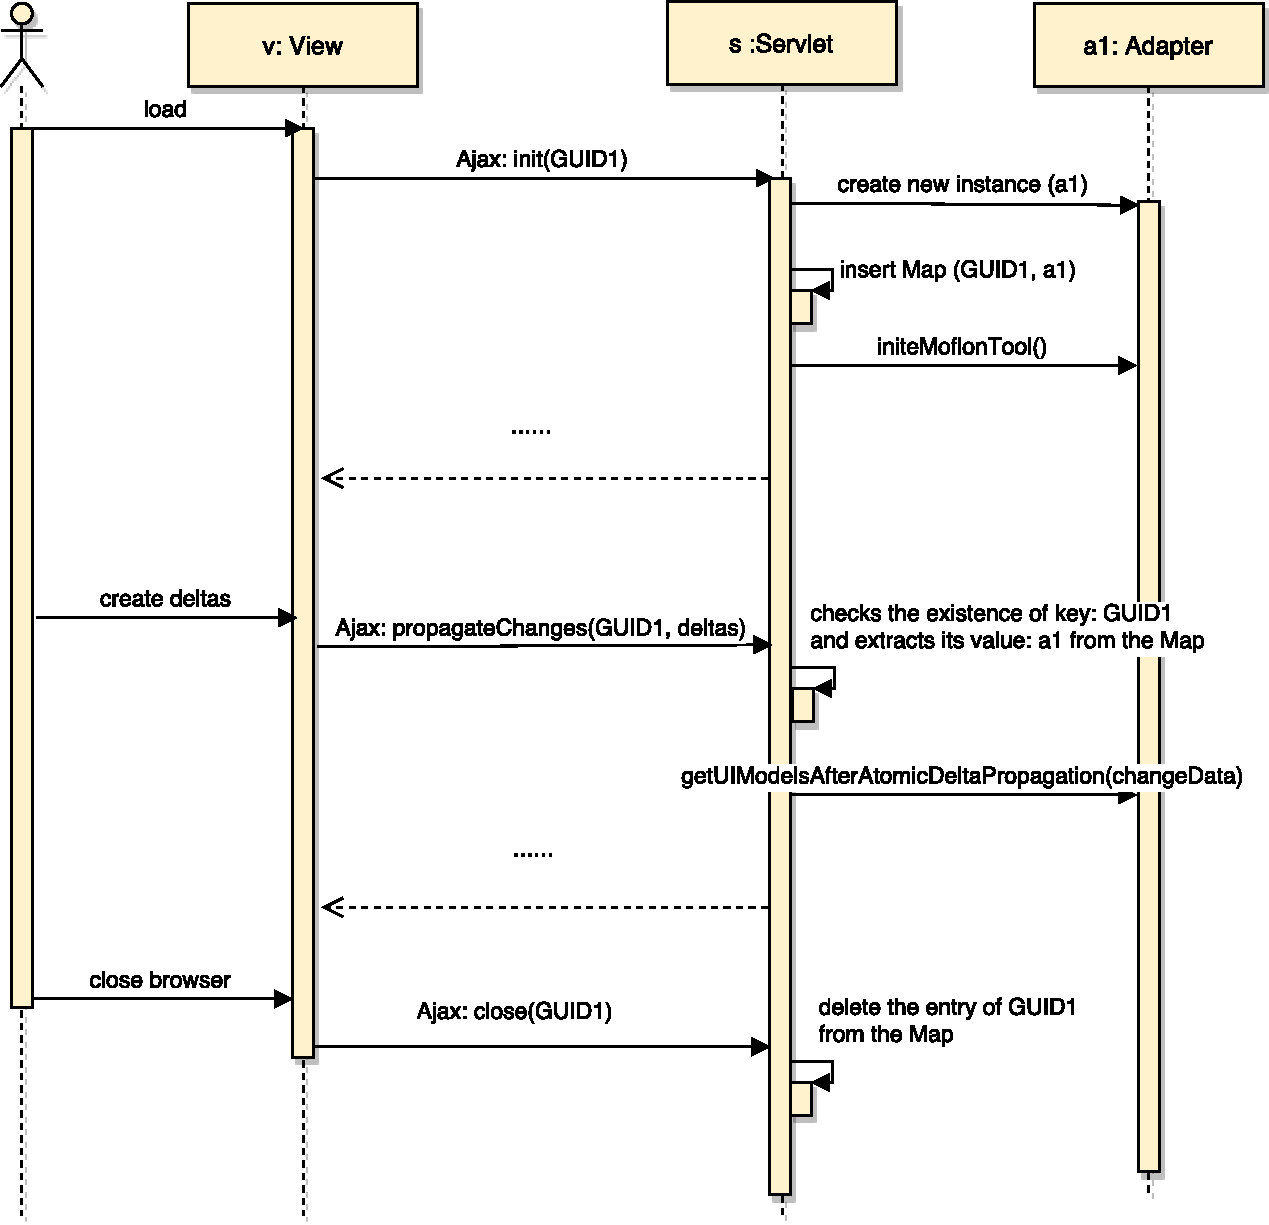
\includegraphics[width=1\textwidth]{figures/Sequence_Diagram-GUID}
	\caption{Sequence Diagram showing the flow of the Unique User id (GUID)}
	\label{fig:Sequence_Diagram-GUID}
\end{figure}
